%%%%%%%%%%%%%%%%%%%%%%%%%%%%%%%%%%%%%%%%%
% Classicthesis Typographic Thesis
% LaTeX Template
% Version 1.4 (1/1/16)
%
% This template has been downloaded from:
% http://www.LaTeXTemplates.com
%
% Original author:
% André Miede (http://www.miede.de) with commenting modifications by:
% Vel (vel@LaTeXTemplates.com)
%
% License:
% GNU General Public License (v2)
%
% General Tips:
% 1) Make sure to edit the classicthesis-config.file
% 2) New enumeration (A., B., C., etc in small caps): \begin{aenumerate} \end{aenumerate}
% 3) For margin notes: \marginpar or \graffito{}
% 4) Do not use bold fonts in this style, it is designed around them
% 5) Use tables as in the examples
% 6) See classicthesis-preamble.sty for useful commands
%
%%%%%%%%%%%%%%%%%%%%%%%%%%%%%%%%%%%%%%%%%

%----------------------------------------------------------------------------------------
%	PACKAGES AND OTHER DOCUMENT CONFIGURATIONS
%----------------------------------------------------------------------------------------

\documentclass[
		twoside,openright,titlepage,numbers=noenddot,headinclude,%1headlines,
	 	footinclude=true,cleardoublepage=empty,
		dottedtoc, % Make page numbers in the table of contents flushed right with dots leading to them
		BCOR=2mm,paper=a4,fontsize=10pt, % Binding correction, paper type and font size
		ngerman,dutch, % Languages, change this to your language(s)
		]{scrreprt}

% Includes the file which contains all the document configurations and packages - make sure to edit this file
%%%%%%%%%%%%%%%%%%%%%%%%%%%%%%%%%%%%%%%%%
% Classicthesis Typographic Thesis
% Configuration File
%
% This file has been downloaded from:
% http://www.LaTeXTemplates.com
%
% Original author:
% André Miede (http://www.miede.de) with extensive commenting changes by:
% Vel (vel@LaTeXTemplates.com)
%
% License:
% GNU General Public License (v2)
%
% Important note:
% The main lines to change in this file are in the DOCUMENT VARIABLES
% section, the rest of the file is for advanced configuration.
%
%%%%%%%%%%%%%%%%%%%%%%%%%%%%%%%%%%%%%%%%%

%----------------------------------------------------------------------------------------
%	CHARACTER ENCODING
%----------------------------------------------------------------------------------------

\PassOptionsToPackage{utf8}{inputenc} % Set the encoding of your files. UTF-8 is the only sensible encoding nowadays. If you can't read äöüßáéçèê∂åëæƒÏ€ then change the encoding setting in your editor, not the line below. If your editor does not support utf8 use another editor!
\usepackage{inputenc}

\usepackage[dutch]{babel}
\selectlanguage{dutch}

%----------------------------------------------------------------------------------------
%	DOCUMENT VARIABLES
%	Fill in the lines below to enter your information into the thesis template
%	Each of the commands can be cited anywhere in the thesis
%----------------------------------------------------------------------------------------

% Remove drafting to get rid of the '[ Date - classicthesis version 4.0 ]' text at the bottom of every page
\PassOptionsToPackage{eulerchapternumbers,listings,drafting, pdfspacing, subfig,beramono,eulermath,parts}{classicthesis}
% Available options: drafting parts nochapters linedheaders eulerchapternumbers beramono eulermath pdfspacing minionprospacing tocaligned dottedtoc manychapters listings floatperchapter subfig

\newcommand{\myTitle}{Analysing SOUP\xspace}
\newcommand{\mySubtitle}{Een weg naar veiligere software\xspace}
\newcommand{\myDegree}{Doktor-Ingenieur (Dr.-Ing.)\xspace}
\newcommand{\myName}{Bas Brunink\xspace}
\newcommand{\myProf}{Bas Breier\xspace}
\newcommand{\myOtherProf}{Marc Grootjen\xspace}
\newcommand{\mySupervisor}{Marc Grootjen\xspace}
\newcommand{\myFaculty}{FDMCI\xspace}
\newcommand{\myDepartment}{Software Engineering\xspace}
\newcommand{\myUni}{Hogeschool van Amsterdam\xspace}
\newcommand{\myLocation}{Amsterdam \xspace}
\newcommand{\myTime}{Februari 2022\xspace}
\newcommand{\myVersion}{version 0.1\xspace}

%----------------------------------------------------------------------------------------
%	USEFUL COMMANDS
%----------------------------------------------------------------------------------------

\newcommand{\ie}{i.\,e.}
\newcommand{\Ie}{I.\,e.}
\newcommand{\eg}{e.\,g.}
\newcommand{\Eg}{E.\,g.} 

\newcounter{dummy} % Necessary for correct hyperlinks (to index, bib, etc.)
\providecommand{\mLyX}{L\kern-.1667em\lower.25em\hbox{Y}\kern-.125emX\@}
\newlength{\abcd} % for ab..z string length calculation

%----------------------------------------------------------------------------------------
%	PACKAGES
%----------------------------------------------------------------------------------------

\usepackage{lipsum} % Used for inserting dummy 'Lorem ipsum' text into the template

%------------------------------------------------

%\PassOptionsToPackage{ngerman,american}{babel}  % Change this to your language(s)
% Spanish languages need extra options in order to work with this template
%\PassOptionsToPackage{spanish,es-lcroman}{babel}
\usepackage{babel}

%------------------------------------------------			

\usepackage{csquotes}
\PassOptionsToPackage{%
%backend=biber, % Instead of bibtex
backend=bibtex8,bibencoding=ascii,%
language=auto,%
style=numeric-comp,%
%style=authoryear-comp, % Author 1999, 2010
%bibstyle=authoryear,dashed=false, % dashed: substitute rep. author with ---
sorting=nyt, % name, year, title
maxbibnames=10, % default: 3, et al.
%backref=true,%
natbib=true % natbib compatibility mode (\citep and \citet still work)
}{biblatex}
\usepackage{biblatex}
 
 %------------------------------------------------

\PassOptionsToPackage{fleqn}{amsmath} % Math environments and more by the AMS 
 \usepackage{amsmath}
 
 %------------------------------------------------

\PassOptionsToPackage{T1}{fontenc} % T2A for cyrillics
\usepackage{fontenc}

%------------------------------------------------

\usepackage{textcomp} % Fix warning with missing font shapes

%------------------------------------------------

\usepackage{scrhack} % Fix warnings when using KOMA with listings package  

%------------------------------------------------

\usepackage{xspace} % To get the spacing after macros right

%------------------------------------------------

\usepackage{mparhack} % To get marginpar right

%------------------------------------------------

\usepackage{fixltx2e} % Fixes some LaTeX stuff 

%------------------------------------------------

\PassOptionsToPackage{smaller}{acronym} % Include printonlyused in the first bracket to only show acronyms used in the text
\usepackage{acronym} % Nice macros for handling all acronyms in the thesis

%\renewcommand*{\acsfont}[1]{\textssc{#1}} % For MinionPro
\renewcommand*{\aclabelfont}[1]{\acsfont{#1}}

%------------------------------------------------

\PassOptionsToPackage{pdftex}{graphicx}
\usepackage{graphicx} 

%----------------------------------------------------------------------------------------
%	FLOATS: TABLES, FIGURES AND CAPTIONS SETUP
%----------------------------------------------------------------------------------------

\usepackage{tabularx} % Better tables
\setlength{\extrarowheight}{3pt} % Increase table row height
\newcommand{\tableheadline}[1]{\multicolumn{1}{c}{\spacedlowsmallcaps{#1}}}
\newcommand{\myfloatalign}{\centering} % To be used with each float for alignment
\usepackage{caption}
\captionsetup{font=small}
\usepackage{subfig}  

%----------------------------------------------------------------------------------------
%	CODE LISTINGS SETUP
%----------------------------------------------------------------------------------------

\usepackage{listings} 
%\lstset{emph={trueIndex,root},emphstyle=\color{BlueViolet}}%\underbar} % For special keywords
\lstset{language=[LaTeX]Tex,%C++ % Specify the language(s) for listings here
morekeywords={PassOptionsToPackage,selectlanguage},
keywordstyle=\color{RoyalBlue}, % Add \bfseries for bold
basicstyle=\small\ttfamily, % Makes listings a smaller font size and a different font
%identifierstyle=\color{NavyBlue}, % Color of text inside brackets
commentstyle=\color{Green}\ttfamily, % Color of comments
stringstyle=\rmfamily, % Font type to use for strings
numbers=left, % Change left to none to remove line numbers
numberstyle=\scriptsize, % Font size of the line numbers
stepnumber=5, % Increment of line numbers
numbersep=8pt, % Distance of line numbers from code listing
showstringspaces=false, % Sets whether spaces in strings should appear underlined
breaklines=true, % Force the code to stay in the confines of the listing box
%frameround=ftff, % Uncomment for rounded frame
%frame=single, % Frame border - none/leftline/topline/bottomline/lines/single/shadowbox/L
belowcaptionskip=.75\baselineskip % Space after the "Listing #: Desciption" text and the listing box
}

%----------------------------------------------------------------------------------------
%	HYPERREFERENCES
%----------------------------------------------------------------------------------------

\PassOptionsToPackage{pdftex,hyperfootnotes=false,pdfpagelabels}{hyperref}
\usepackage{hyperref}  % backref linktocpage pagebackref
\pdfcompresslevel=9
\pdfadjustspacing=1

\hypersetup{
% Uncomment the line below to remove all links (to references, figures, tables, etc), useful for b/w printouts
%draft, 
colorlinks=true, linktocpage=true, pdfstartpage=3, pdfstartview=FitV,
% Uncomment the line below if you want to have black links (e.g. for printing black and white)
%colorlinks=false, linktocpage=false, pdfborder={0 0 0}, pdfstartpage=3, pdfstartview=FitV, 
breaklinks=true, pdfpagemode=UseNone, pageanchor=true, pdfpagemode=UseOutlines,%
plainpages=false, bookmarksnumbered, bookmarksopen=true, bookmarksopenlevel=1,%
hypertexnames=true, pdfhighlight=/O,%nesting=true,%frenchlinks,%
urlcolor=webbrown, linkcolor=RoyalBlue, citecolor=webgreen, %pagecolor=RoyalBlue,%
    %urlcolor=Black, linkcolor=Black, citecolor=Black, %pagecolor=Black,%
%------------------------------------------------
% PDF file meta-information
pdftitle={\myTitle},
pdfauthor={\textcopyright\ \myName, \myUni, \myFaculty},
pdfsubject={},
pdfkeywords={},
pdfcreator={pdfLaTeX},
pdfproducer={LaTeX with hyperref and classicthesis}
%------------------------------------------------
}

%----------------------------------------------------------------------------------------
%	AUTOREFERENCES SETUP
%	Redefines how references in text are prefaced for different 
%	languages (e.g. "Section 1.2" or "section 1.2")
%----------------------------------------------------------------------------------------

\makeatletter
\@ifpackageloaded{babel}
{
\addto\extrasamerican{
\renewcommand*{\figureautorefname}{Figure}
\renewcommand*{\tableautorefname}{Table}
\renewcommand*{\partautorefname}{Part}
\renewcommand*{\chapterautorefname}{Chapter}
\renewcommand*{\sectionautorefname}{Section}
\renewcommand*{\subsectionautorefname}{Section}
\renewcommand*{\subsubsectionautorefname}{Section}
}
\addto\extrasngerman{
\renewcommand*{\paragraphautorefname}{Absatz}
\renewcommand*{\subparagraphautorefname}{Unterabsatz}
\renewcommand*{\footnoteautorefname}{Fu\"snote}
\renewcommand*{\FancyVerbLineautorefname}{Zeile}
\renewcommand*{\theoremautorefname}{Theorem}
\renewcommand*{\appendixautorefname}{Anhang}
\renewcommand*{\equationautorefname}{Gleichung}
\renewcommand*{\itemautorefname}{Punkt}
}
\providecommand{\subfigureautorefname}{\figureautorefname} % Fix to getting autorefs for subfigures right
}{\relax}
\makeatother

%----------------------------------------------------------------------------------------

\usepackage{classicthesis} 

%----------------------------------------------------------------------------------------
%	CHANGING TEXT AREA 
%----------------------------------------------------------------------------------------

%\linespread{1.05} % a bit more for Palatino
%\areaset[current]{312pt}{761pt} % 686 (factor 2.2) + 33 head + 42 head \the\footskip
%\setlength{\marginparwidth}{7em}%
%\setlength{\marginparsep}{2em}%

%----------------------------------------------------------------------------------------
%	USING DIFFERENT FONTS
%----------------------------------------------------------------------------------------

%\usepackage[oldstylenums]{kpfonts} % oldstyle notextcomp
%\usepackage[osf]{libertine}
%\usepackage[light,condensed,math]{iwona}
%\renewcommand{\sfdefault}{iwona}
%\usepackage{lmodern} % <-- no osf support :-(
%\usepackage{cfr-lm} % 
%\usepackage[urw-garamond]{mathdesign} <-- no osf support :-(
%\usepackage[default,osfigures]{opensans} % scale=0.95 
%\usepackage[sfdefault]{FiraSans}

\addbibresource{Bibliography.bib} % The file housing your bibliography
%\addbibresource[label=ownpubs]{Self_Publications.bib} % Uncomment for optional self-publications

%\hyphenation{Put special hyphenation here}


\begin{document}

\frenchspacing % Reduces space after periods to make text more compact

\raggedbottom % Makes all pages the height of the text on that page

\selectlanguage{dutch} % Select your default language - e.g. american or ngerman

%\renewcommand*{\bibname}{new name} % Uncomment to change the name of the bibliography
%\setbibpreamble{} % Uncomment to include a preamble to the bibliography - some text before the reference list starts

\pagenumbering{roman} % Roman page numbering prior to the start of the thesis content (i, ii, iii, etc)

\pagestyle{plain} % Suppress headers for the pre-content pages

%----------------------------------------------------------------------------------------
%	PRE-CONTENT THESIS PAGES
%----------------------------------------------------------------------------------------

% Title Page

\begin{titlepage}

\begin{addmargin}[-1cm]{-3cm}
\begin{center}
\large

\hfill
\vfill

\begingroup
\color{Maroon}\spacedallcaps{\myTitle} \\ \bigskip % Thesis title
\endgroup

\spacedlowsmallcaps{\myName} % Your name

\vfill

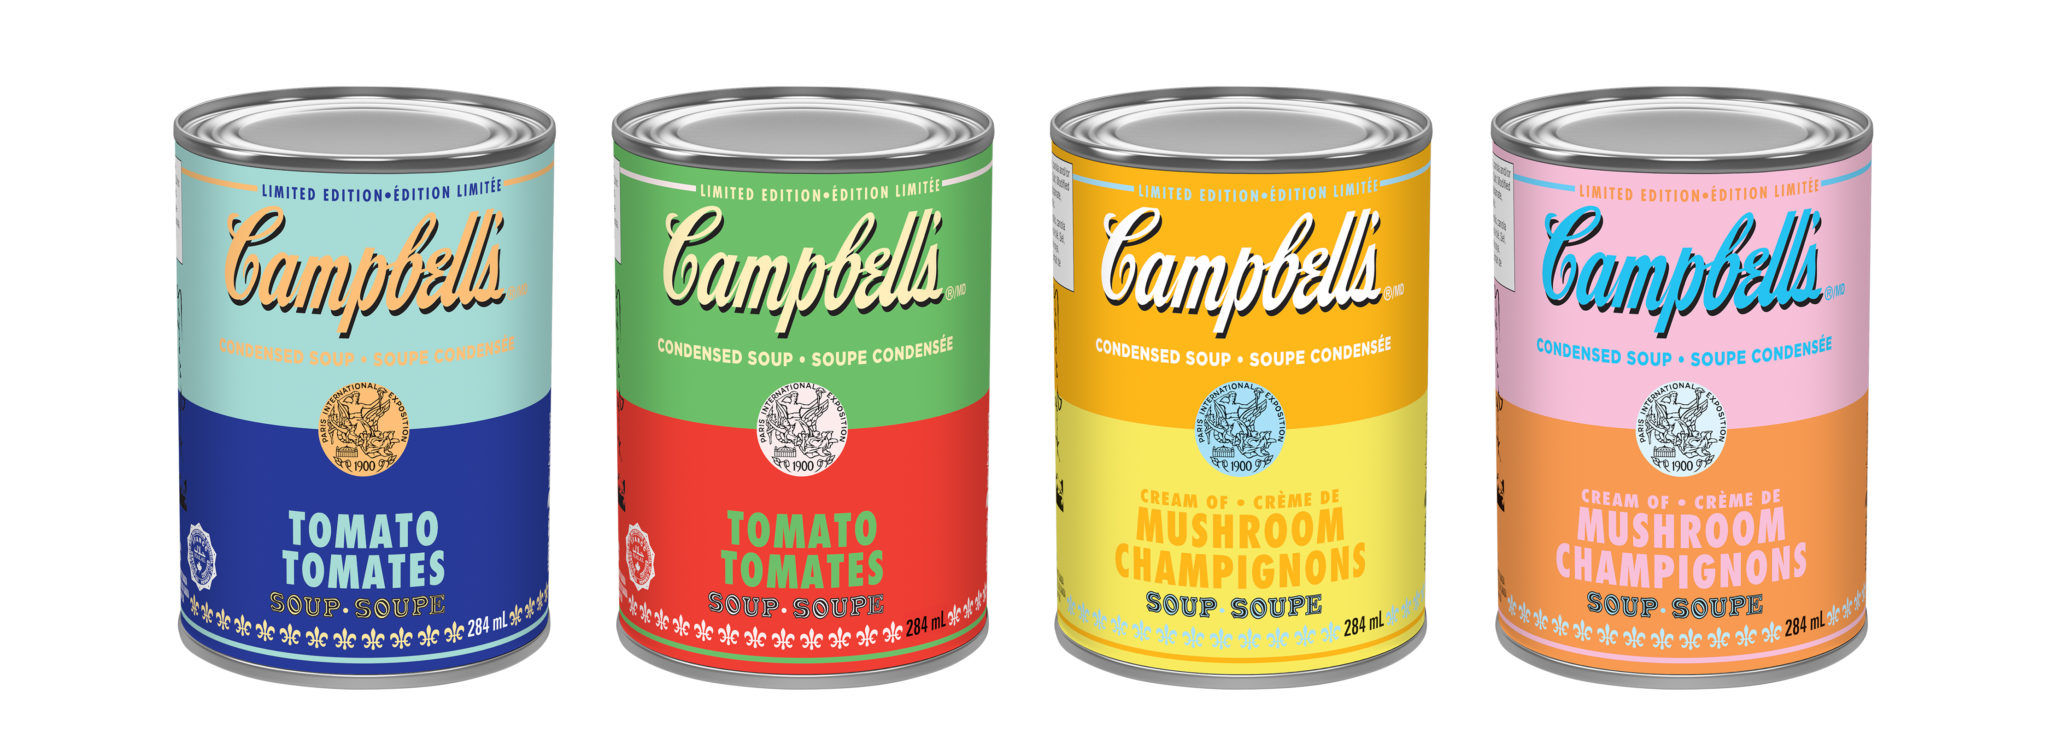
\includegraphics[width=10cm]{gfx/soupcans} \\ \medskip % Picture

\mySubtitle \\ \medskip % Thesis subtitle
%\myDegree \\
\myDepartment \\
\myFaculty \\
\myUni \\ \bigskip

\myTime\ -- \myVersion % Time and version

\vfill

\end{center}
\end{addmargin}

\end{titlepage} % Main title page

% Back of the title page

\thispagestyle{empty}

\hfill

\vfill

\noindent\myName: \textit{\myTitle,} \mySubtitle, %\myDegree, 
\textcopyright\ \myTime

% You may wish to do something with the back of the title page, such as including your supervisors, location or time frame of the work. Below is an example of doing so although you may want to tweak it to your liking.

%\bigskip

%\noindent\spacedlowsmallcaps{Supervisors}: \\
%\myProf \\
%\myOtherProf \\ 
%\mySupervisor

%\medskip \\

%\noindent\spacedlowsmallcaps{Location}: \\
%\myLocation

%\medskip \\

%\noindent\spacedlowsmallcaps{Time Frame}: \\
%\myTime
 % Back of the title page

%\cleardoublepage% Dedication

\thispagestyle{empty}
\refstepcounter{dummy}

\pdfbookmark[1]{Dedication}{Dedication} % Bookmark name visible in a PDF viewer

\vspace*{3cm}

\begin{center}
\emph{Ohana} means family. \\
Family means nobody gets left behind, or forgotten. \\ \medskip
--- Lilo \& Stitch    
\end{center}

\medskip

\begin{center}
Dedicated to the loving memory of Rudolf Miede. \\ \smallskip
1939\,--\,2005
\end{center} % Dedication page

%\cleardoublepage\include{FrontBackMatter/Foreword} % Uncomment and create a Foreword.tex to include a foreword

\cleardoublepage% Abstract

%\renewcommand{\abstractname}{Abstract} % Uncomment to change the name of the abstract

\pdfbookmark[1]{Abstract}{Abstract} % Bookmark name visible in a PDF viewer

\begingroup
\let\clearpage\relax
\let\cleardoublepage\relax
\let\cleardoublepage\relax

\chapter*{Abstract}
Short summary of the contents\dots a great guide by 
Kent Beck how to write good abstracts can be found here:  
\begin{center}
\url{https://plg.uwaterloo.ca/~migod/research/beckOOPSLA.html}
\end{center}

\endgroup			

\vfill % Abstract page

%\cleardoublepage% Publications - a page listing research articles written using content in the thesis

\pdfbookmark[1]{Publications}{Publications} % Bookmark name visible in a PDF viewer

\chapter*{Publications} % Publications page text

Some ideas and figures have appeared previously in the following publications:\\

\noindent Put your publications from the thesis here. The packages \texttt{multibib} or \texttt{bibtopic} etc. can be used to handle multiple different bibliographies in your document.

%\begin{refsection}[ownpubs]
%    \small
%    \nocite{*} % is local to to the enclosing refsection
%    \printbibliography[heading=none]
%\end{refsection}

%\emph{Attention}: This requires a separate run of \texttt{bibtex} for your \texttt{refsection}, \eg, \texttt{ClassicThesis1-blx} for this file. You might also use \texttt{biber} as the backend for \texttt{biblatex}. See also \url{http://tex.stackexchange.com/questions/128196/problem-with-refsection}. % Publications from the thesis page

%\cleardoublepage\usepackage{natbib}% Acknowledgements

\pdfbookmark[1]{Acknowledgements}{Acknowledgements} % Bookmark name visible in a PDF viewer

\begin{flushright}{\slshape
We have seen that computer programming is an art, \\
because it applies accumulated knowledge to the world, \\
because it requires skill and ingenuity, and especially \\
because it produces objects of beauty.} \\ \medskip
--- \defcitealias{knuth:1974}{Donald E. Knuth}\citetalias{knuth:1974} \citep{knuth:1974}
\end{flushright}

\bigskip

%----------------------------------------------------------------------------------------

\begingroup

\let\clearpage\relax
\let\cleardoublepage\relax
\let\cleardoublepage\relax

\chapter*{Acknowledgements}

\noindent Put your acknowledgements here.\\

\noindent Many thanks to everybody who already sent me a postcard!\\

\noindent Regarding the typography and other help, many thanks go to Marco Kuhlmann, Philipp Lehman, Lothar Schlesier, Jim Young, Lorenzo Pantieri and Enrico Gregorio\footnote{Members of GuIT (Gruppo Italiano Utilizzatori di \TeX\ e \LaTeX )}, J\"org Sommer, Joachim K\"ostler, Daniel Gottschlag, Denis Aydin, Paride Legovini, Steffen Prochnow, Nicolas Repp, Hinrich Harms, Roland Winkler, and the whole \LaTeX-community for support, ideas and some great software.

\bigskip

\noindent\emph{Regarding \mLyX}: The \mLyX\ port was initially done by
\emph{Nicholas Mariette} in March 2009 and continued by
\emph{Ivo Pletikosi\'c} in 2011. Thank you very much for your work and the contributions to the original style.

\endgroup
 % Acknowledgements page

\pagestyle{scrheadings} % Show chapter titles as headings

\cleardoublepage% Table of Contents - List of Tables/Figures/Listings and Acronyms

\refstepcounter{dummy}

\pdfbookmark[1]{\contentsname}{tableofcontents} % Bookmark name visible in a PDF viewer

\setcounter{tocdepth}{2} % Depth of sections to include in the table of contents - currently up to subsections

\setcounter{secnumdepth}{3} % Depth of sections to number in the text itself - currently up to subsubsections

\manualmark
\markboth{\spacedlowsmallcaps{\contentsname}}{\spacedlowsmallcaps{\contentsname}}
\tableofcontents
\automark[section]{chapter}
\renewcommand{\chaptermark}[1]{\markboth{\spacedlowsmallcaps{#1}}{\spacedlowsmallcaps{#1}}}
\renewcommand{\sectionmark}[1]{\markright{\thesection\enspace\spacedlowsmallcaps{#1}}}

\clearpage

\begingroup
\let\clearpage\relax
\let\cleardoublepage\relax
\let\cleardoublepage\relax

%----------------------------------------------------------------------------------------
%	List of Figures
%----------------------------------------------------------------------------------------

\refstepcounter{dummy}
%\addcontentsline{toc}{chapter}{\listfigurename} % Uncomment if you would like the list of figures to appear in the table of contents
\pdfbookmark[1]{\listfigurename}{lof} % Bookmark name visible in a PDF viewer

\listoffigures

\vspace{8ex}
\newpage

%----------------------------------------------------------------------------------------
%	List of Tables
%----------------------------------------------------------------------------------------

%\refstepcounter{dummy}
%%\addcontentsline{toc}{chapter}{\listtablename} % Uncomment if you would like the list of tables to appear in the table of contents
%\pdfbookmark[1]{\listtablename}{lot} % Bookmark name visible in a PDF viewer
%
%\listoftables
%
%\vspace{8ex}
%\newpage
%
%%----------------------------------------------------------------------------------------
%	List of Listings
%----------------------------------------------------------------------------------------

\refstepcounter{dummy}
%\addcontentsline{toc}{chapter}{\lstlistlistingname} % Uncomment if you would like the list of listings to appear in the table of contents
\pdfbookmark[1]{\lstlistlistingname}{lol} % Bookmark name visible in a PDF viewer

\lstlistoflistings

\vspace{8ex}
\newpage

%----------------------------------------------------------------------------------------
%	Acronyms
%----------------------------------------------------------------------------------------

\refstepcounter{dummy}
%\addcontentsline{toc}{chapter}{Acronyms} % Uncomment if you would like the acronyms to appear in the table of contents
\pdfbookmark[1]{Acronyms}{acronyms} % Bookmark name visible in a PDF viewer

\markboth{\spacedlowsmallcaps{Acronyms}}{\spacedlowsmallcaps{Acronyms}}

\chapter*{Acroniemen}

\begin{acronym}[UML]
\acro{API}{Application Programming Interface}
\acro{CEO}{Chief Executive Officer}
\acro{CFO}{Chief Financial Officer}
\acro{COO}{Chief Operations Officer}
\acro{CTO}{Chief Technology Officer}
\acro{CI/CD}{Continuous Integration - Continuous Delivery/Deployment}
\acro{CVE}{Common Vulnerabilities and Exposures}
\acro{CSRC}{Computer Security Research Center (onderdeel van NIST)}
\acro{NIST}{National Institute of Standards and Technology}
\acro{OSS}{Open Source Software}
\acro{OTAP}{Ontwikkeling Test Acceptatie Productie}
\acro{SOUP}{Software of Unkown Pedigree / Provenance}
\acro{MT}{Management team}
\acro{MoSCoW}{Must, Should, Could, Won't Have (zie begrippenlijst voor uitleg)}
\acro{UML}{Unified Modeling Language}
\end{acronym}

\endgroup
 % Contents, list of figures/tables/listings and acronyms

\cleardoublepage

\pagenumbering{arabic} % Arabic page numbering for thesis content (1, 2, 3, etc)
%\setcounter{page}{90} % Uncomment to manually start the page counter at an arbitrary value (for example if you wish to count the pre-content pages in the page count)

\cleardoublepage % Avoids problems with pdfbookmark

%----------------------------------------------------------------------------------------
%	THESIS CONTENT - CHAPTERS
%----------------------------------------------------------------------------------------

% Text on the Part 1 page describing  the content in Part 1

\chapter{Inleiding} % Chapter title

\label{ch:Inleiding} % For referencing the chapter elsewhere, use \autoref{ch:introduction} 
Het document dat voor u ligt is een resultaat van een onderzoek en product oplevering als afstudeeropdracht door Bas Brunink voor het bedrijf Eaglescience. Het zal het process beschrijven die ik gelopen heb om een module te schrijven die automatisch een SOUP analyse doet op zowel bestaande als nieuwe projecten. 

\section{leeswijzer}
Deze scriptie neemt de lezer mee door het verloop van het project van idee tot implementatie. Met als einde een resultaat beschrijven en een prognose in de verbetering gezien de verwachting is dat er niet direct een significante verbetering te zien is.  % inleiding

\ctparttext{}

\part{Opdracht} % First part of the thesis
% Chapter 1
\chapter{Eaglescience} % Chapter title

\label{ch:Eaglescience} % For referencing the chapter elsewhere, use \autoref{ch:introduction}

%----------------------------------------------------------------------------------------

Het hier beschreven onderzoek en de daarbij behorende applicatie is geschreven in opdracht van het bedrijf Eaglescience wat gevestigd is in Amsterdam Sloterdijk. Eaglescience ontwikkeld complexe software op projectbasis voor diverse klanten. Deze projecten hebben vaak een wetenschappelijke inslag. Hiernaast biedt Eaglescience ook de mogelijkheid aan de klant om zorg te dragen voor de eventuele hosting van het opgeleverde product. Eaglescience kan hierdoor nog beter garanderen dat de geboden kwaliteit in de software gewaarborgd blijft tijdens de levensduur van de software.

\section{Organisatie}
\marginpar{Organisatie}

Eaglescience BV bestaat uit drie divisies: Innovations, Software en Solutions [figuurX]: %besxchrijving van de drie takken
Het bestaat op het moment van schrijven uit $\pm$ 20 medewerkers waarvan 75\% verantwoordelijk is voor de ontwikkeling van de geleverde software. De andere 25\% bekleed een support rol zoals project manager, finance manager, quality manager, automatisering etc. \\

\begin{figure}[bth]
\myfloatalign
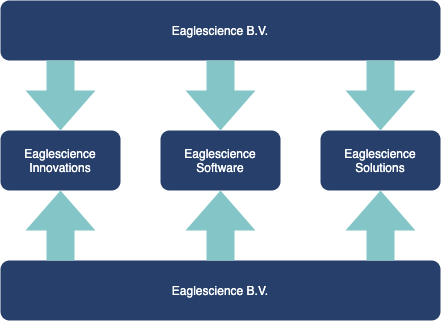
\includegraphics[width=10cm]{gfx/organogram}
\caption{Organogram Eaglescience}
\label{fig:Eaglescience organogram}
\end{figure}
% vragen Wat zijn de hoofddoelen van iedere divisie?
% betere verwoording vragen:
De divisie Eaglescience Innovations zoekt naar nieuwe oplossingen op het gebied van software ontwikkeling, deze worden door de divisie  Eaglescience software ge\"implementeert. Eaglescience Solutions is een divisie die samen met de klant opzoek gaat naareen oplossing voor een gesteld probleem.\\
Het dagelijks bestuur is handen van:
\begin{itemize}
\item CEO/CFO - Marc Grootjen
\item CTO - Bas Breier
\item COO - Wender van Mansvelt \\
\end{itemize}
Onder het dagelijks bestuur valt Team Eaglescience wat bestaat uit projectmanagers en ontwikkelaars. Deze zijn onderverdeeld in diverse scrum teams die ieders verantwoordelijk zijn voor een project. De ontwikkelaars worden parallel ingezet op meerdere projecten om kennisdeling te bevorderen.

\section{missie}
\marginpar{missie}
De missie van Eaglescience is het bedienen van haar partners door een ontwerp, ontwikkeling en service te bieden op het gebied van op maat gemaakte IT oplossingen . Om dit te kunnen bewerkstelligen heeft Eaglescience goed opgeleide IT professionals in dienst die zichzelf continue ontwikkelen op de “cutting edge” van IT technologie. De hoofd competenties van de medewerkers zijn: innovatief, intelligent, klant georientee\"erd, flexibel en ambitieus.

\section{visie}
Eaglescience streeft er als innovatief IT bedrijf naar om software te ontwikkelen als een Business-to-Business dienst. Met onze technische vaardigheden bouwen we veilige en hoogwaardige software die bijdraagt aan een betere wereld. Omdat we agile werken, leveren we precies wat nodig is, niets meer en niets minder. Wij helpen onze klanten zoeken naar een langdurige betrokkenheid en samenwerking op basis van zowel vertrouwen als wederzijds respect. \\
\marginpar{visie}
Omdat elke vraag uniek is, ontwikkeld Eaglescience op maar gemaakte en innovatieve software. We zijn van plan deel uit te maken van het hele proces van het formuleren van een idee tot het lanceren van het product en het waarborgen van de productie levenscyclus. Onze belangrijkste succesfactor zijn de mensen, die zich continu ontwikkelen door met de nieuwste technieken te werken op diverse projecten. Wij streven naar een optimale balans tussen werk en priv\'e. Dit geeft onze medewerkers veel vrijheid, maar vereist zelfdiscipline en verantwoordelijkheid.

\section{strategie}
Eaglescience levert de visie via vier strategische thema's:
\begin{itemize}
\item Maatschappelijke verantwoordelijkheid
\item Persoonlijke groei
\item Tevredenheid
\item 4e???? %hbjvjhbjb
\end{itemize}
\marginpar{strategische thema's}
We streven ernaar om veilige en hoogwaardige software diensten te leveren die waarde toevoegen aan onze samenleving. We streven naar een bedrijfscultuur waarin alle collega's hun talenten kunnen laten groeien. We hebben een ongecompliceerd werkethos: we richten ons op resultaten van hoge kwaliteit, maar met een gezonde balans tussen werk en priv\'e en voldoende tijd voor leuke en sociale evenementen. Eaglescience verwacht van alle medewerkers dat zij hun handelen baseren op vier kwaliteitsprincipes:
\begin{itemize}
\item Meld situaties die niet voldoen aan onze interne procedures
\item Evalueer risico's wanneer grote veranderingen worden verwacht
\item Help en daag elkaar uit
\item Kennis behouden over compliancy en kwaliteitsmanagement
\end{itemize}

\section{Werkwijze}
Zoals eerder gemeld werkt Eaglescience op projectbasis met ontwikkelaars in meedere teams. Er wordt getracht "Full scrum "te werken waarbij de requirements van de klant centraal staan. Als een project wordt aangenomen door het management team dan wordt deze in sprints in samenwerking met de klant ontwikkeld. De klant wordt nauw betrokken bij het verloop van de ontwikkeling door middel van demo's aan het einde van iedere sprint, hier wordt gemeten hoe de applicatie zich gedraagt met betrekking tot de requirements van de klant. Dit is ook het moment dat er feedback gegeven wordt en waar waar nodig gestuurd kan worden in het verdere verloop. Op het moment dat er een applicatie klaar is wordt de software dan al niet overgedragen aan de klant of door gegeven aan support en hosting die verantwoordelijk zijn voor de daadwerkelijke hosting van de software.
\begin{figure}[bth]
\myfloatalign
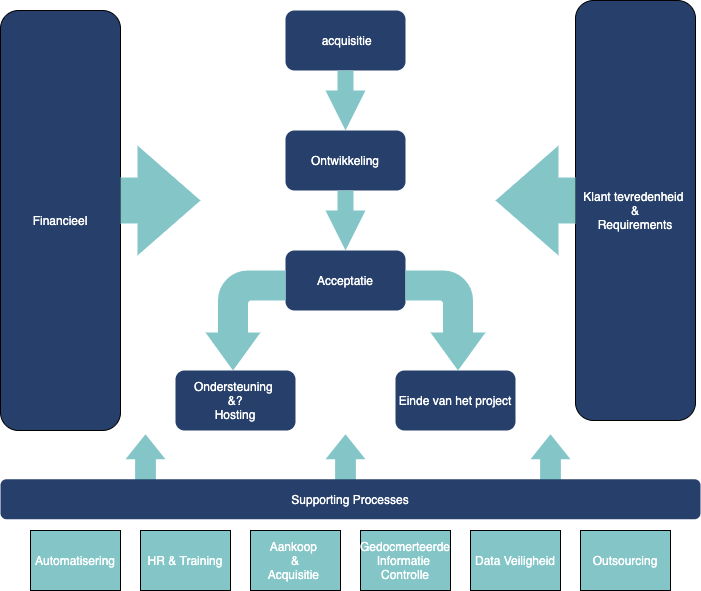
\includegraphics[width=10cm]{gfx/ProcessFlow}
\caption{Project Process}
\label{fig:Project Process}
\end{figure}
Naast het ontwikkel process zijn er een aantal supporting processes die ervoor zorgdragen dat het bedrijf blijft draaien en er nieuwe mensen aangenomen worden, maar ook een deel automatisering die voor ondersteuning zorgt voor platformen waarop ontwikkeld en of gehosted wordt.\\
Eaglescience ontwikkeld op projectbasis en op die manier komen er ook inkomsten. Dus alle processen die draaien moeten ingezet kunnen worden op projecten van klanten. Als er een project voor in huis gebruik wordt ondernomen moet er een duidelijk beeld zijn of er op termijn winst mee te behalen is op monetair vlak dan al niet tijdswinst of ontwikkel gemak.

\section{}

\section{Relevante en actuele ontwikkelingen binnen Eaglescience}
Eaglescience is aan het groeien, zowel in het aantal projecten waar aan gewerkt wordt als het aantal medewerkers. Daarnaast worden de diensten die Eaglescience aanbied ook uitgebreid. Waarbij het hosten van de ontwikkelde applicaties steeds meer wordt aangeboden. Door deze inzet ligt de verantwoordelijk niet alleen bij het leveren van een veilige en hoogwaardige software maar het leveren van service waarbij de applicaties in een veilige omgeving worden aangeboden. Mede door de groei van het bedrijf maar zeker ook de diensten die aangeboden wordt is het zeer relevant om taken die geautomatiseerd kunnen worden te automatiseren.
 % Chapter 1 Eaglescience
% Chapter 2

\chapter{Opdracht} % Chapter title
\label{ch:opdracht} % For referencing the chapter elsewhere, use \autoref{ch:examples}
Tegenwoordig zijn software-bibliotheken niet meer weg te denken in het software ontwikkelproces van nu. Bibliotheken geven ontwikkelaars de mogelijkheid code her te gebruiken in meerdere projecten om zo effici\"enter te kunnen ontwikkelen. Wat op zijn beurt weer meehelpt om de Time-To-Market te verkorten. Bibliotheken kunnen door bedrijven zelf geschreven worden, in het geval van EagseScience is dit Arches, of worden overgenomen van andere bedrijven/instellingen. Zelfs Arches is afhankelijk van een aantal bibliotheken die niet ontwikkeld zijn door Eaglescience. Dus ontkom je er tegenwoordig niet aan om bibliotheken te gebruiken waarvan je de afkomst niet geheel kan herleiden.\\
Deze bibliotheken vallen onder de noemer "Software of Unknown Provenance/Pedigree(SOUP)". Door het gebruik van dit soort bibliotheken kan er een aannemelijk risico ontstaan op het gebied van kwetsbaarheden. Om inzicht te krijgen in deze kwetsbaarheden en daarmee dus mogelijk veiligheidsissues dient er een SOUP analyse gedaan worden. Binnen Eaglescience wordt het belang gezien om deze analyse te doen en is daarom op zoek naar een efficiënte en mogelijk geautomatiseerde manier voor het uitvoeren van een dergelijke analyse om zo de veiligheid van de ontwikkelde applicaties te waarborgen zonder afbreuk te doen aan kwaliteit.

\section{Opdracht vanuit Eaglescience}
Vanuit de CTO is de wens ontstaan om een gestructureerde methode te ontwikkelen waarbij er automatisch periodiek een SOUP analyse gedaan wordt op bestaande en nieuwe projecten. Het uiteindelijke resultaat moet zijn dat er een module wordt toegevoegd aan de reeds bestaande portal van Eaglescience waarbij project verantwoordelijken inzicht kunnen verkrijgen in de kwetsbaarheden die in een project aanwezig kunnen zijn door het gebruik van externe bibliotheken.
%------------------------------------------------

\subsection{Eisen aan de opdracht}

Vanuit Eaglescience zijn er een aantal eisen gesteld waaraan het eindproduct moet voldoen. Als er aan deze eisen is voldaan dan is er voor Eaglescience een waardevol product wat men dan ook in gebruik kan nemen. Daarnaast zijn er een aantal oplever eisen die gehaald dienen te worden om de kwaliteit te waarborgen. \\

\textbf{functionele eisen}
\begin{itemize}
\item De module dient eenvoudig te worden gebruikt in de huidige CI/CD pipeline voor bestaande en nieuwe projecten
\item De module dient gebruik te maken van de bestaande ++huidige++ projectstructuur van het portal
\item De module dient ondersteuning te bieden voor meerdere omgevingen(OTAP)
\item De module dient met een instelbaar interval de analyse uit te voeren
\item De module op project en omgeving niveau te rapporteren over bekende kwetsbaarheden
\item De module dient kwetsbaarheden op minimaal drie niveau’s in te schalen (kritisch, gemiddeld en laag)
\item De module dient ondersteuning te bieden voor het instellen van quality gates ten aanzien van ieder niveau, per project, per omgeving
\item De module wordt ontwikkeld in Angular en Play(scala), overeenkomstig bestaande portal modules
\end{itemize}
\textbf{kwaliteitseisen}
\begin{itemize}
\item De module voldoet aan de geldende kwaliteitsnormen binnen Eaglescience, minimaal meetbaar door:
	\begin{itemize}
	\item test coverage > 70\%
	\item onderdeel van de bestaande CI/CD voor het Eaglescience Portal
	\end{itemize}
\item Geschreven code is gereviewd door een Eaglescience ontwikkelaar
\item In de module zijn gescheiden componenten: Frontend, Backend, API onafhankelijk en goed gedocumenteerd.
\item Voor de API documentatie wordt gebruik gemaakt van swagger.
\end{itemize}

\subsection{Deliverables}
Vanuit de CTO zijn er naast de functionele eisen ook eisen gesteld aan de oplevering:
\begin{itemize}
\item Geïntregreerde en aantoonbaar werkende module
\item De code van de module in Eaglsescience GitLab
\item API documentatie (middels swagger)
\item Een handleiding hoe de module gebruikt dient te worden
\item Eventuele aanvullende deliverables vanuit de HvA
\end{itemize}


\section{Opdracht fasen}
Om de hierboven beschreven opdracht zo goed als mogelijk uit te voeren dient er eerst een onderzoek gedaan worden naar het begrippen binnen het domein SOUP en daarnaast mogelijkheden om bibliotheken te screenen/testen op kwetsbaarheden. Daarna moet er een module ontwikkeld worden die deze mogelijkheid implementeerd met in achtneming van de bovengenoemde eisen.
\subsection{Fase 1: Onderzoek}
Als eerste dient er een begrippen/literatuur onderzoek gedaan te worden binnen het domein soup om een goed kennis te vergaren over het domein om zo een basis te leggen voor een te implementeren module. Daarnaast dient er onderzoek gedaan te worden om te zien of er bibliotheken zijn en resources waar informatie of SOUP bibliotheken te vinden is. en aan welke eisen deze moeten voldoen. Hier lettende op de eisen vanuit Eaglescience en de mogelijkheden die deze analyse bibliotheken bieden. Deze fase wordt beschreven in het tweede deel van dit document.

\subsection{Fase 2: Oplevering SOUP analyse module}
De uit het onderzoek behaalde resultaten ten opzicht van beschikbare resources om een SOUP analyse te voeden moet worden geimplementeerd in een module binnen een bestaande applicatie. Deze module dient te voldoen aan de eisen die gesteld zijn. Het ontwerp en implementatie wordt beschreven

\section{plan van aanpak}
Het plan is als volgt:
\begin{enumerate}
\item LiteratuurOnderzoek
\\ Wat gebeurt er als ik hier text plaats
\item Markt onderzoek
\item Resultaat onderzoek
\item ontwerp implementatie
\item Ontwikkeling implementatie
\item Deploy implementatie
\end{enumerate}




\section{mindmap test}
Kijken of dit nog waardevol is : \\

\begin{tikzpicture}[grow cyclic, text width=2.7cm, align=flush center,
	level 1/.style={level distance=5cm,sibling angle=90},
	level 2/.style={level distance=3cm,sibling angle=45}]

\node{ShareLaTeX Tutorial Videos}
child { node {Beginners Series}
	child { node {First Document}}
	child { node {Sections and Paragraphs}}
	child { node {Mathematics}}
	child { node {Images}}
	child { node {bibliography}}
	child { node {Tables and Matrices}}
	child { node {Longer Documents}}
}
child { node {Thesis Series}
	child { node {Basic Structure}}
	child { node {Page Layout}}
	child { node {Figures, Subfigures and Tables}}
	child { node {Biblatex}}
	child { node {Title Page}}
}
child { node {Beamer Series}
	child { node {Getting Started}}
	child { node {Text, Pictures and Tables}}
	child { node {Blocks, Code and Hyperlinks}}
	child { node {Overlay Specifications}}
	child { node {Themes and Handouts}}
}
child { node {TikZ Series}
	child { node {Basic Drawing}}
	child { node {Geogebra}}
	child { node {Flow Charts}}
	child { node {Circuit Diagrams}}
	child { node {Mind Maps}}
};
\end{tikzpicture}
 % Chapter 2 Opdracht
\part{Requirements Analyse en planning}
% Chapter 3

\chapter{Inleiding} % Chapter title

\label{inReqPlan} % For referencing the chapter elsewhere, use \autoref{ch:InReqPlan}
Op basis van de opdracht die in het vorige deel is er een requirements analyse gedaan deze analyse moet inzicht brengen in de vele details die de opdracht heeft. Er zijn gesprekken gevoerd met de CTO en andere stakeholders om te achterhalen welke requirements er zijn. Daarnaast is het belang voor iedere stakeholder geanalyseerd. Als laatst wordt er in grove lijnen een planning gepresenteerd waarin het project is uitgevoerd.


\chapter{Requirements Analyse} % Chapter title

\label{inOnderzoek} % For referencing the chapter elsewhere, use \autoref{ch:InOnderzoek}

\section{huidige situatie}
In de huidige situatie wordt er een SOUP analyse gedaan door de ontwikkelaars op het moment dat een project ontwikkelt wordt. dit is veelal handmatig zoeken in online resources op bibliotheken die gebruikt worden. Dit neemt veel kostbare tijd in beslag die beter besteed kan worden om nieuwe features toe te voegen. Daarnaast worden de bevindingen die gedaan worden niet centraal opgeslagen zodat er een potentie is dat niet iedereen op de hoogte is van de actuele informatie.

\section{De Stakeholders}
De stakeholders kunnen opgedeelt worden in twee groepen(Tabel 1): externe en interne stakeholders.
\begin{table}
%\myfloatalign
\begin{tabularx}{\textwidth}{Xll} \toprule
\tableheadline{Groep}   & \tableheadline{Stakeholder}\\
\midrule
Extern                  & Klant                      \\
\midrule
Intern                  & Dagelijks Bestuur          \\
                        & Project managers           \\
                        & CTO                        \\
                        & Ontwikkelaars              \\
\bottomrule
\end{tabularx}
\caption[Verdeling stakeholders]{Verdeling stakeholders}
\label{tab:verdeling_StakeHolders}
\end{table}

Een deel van de stakeholders zijn geinterviewt om te achterhalen welke verbeteringen zij zien in de nieuwe module.

Verslagen van de interviews zijn te lezen in bijlage X Interviews


\subsection{Dagelijks bestuur (intern) }
De CTO ziet vooral winst in tijd als deze module
\subsection{Klant(extern)}
De klant is een passieve stackeholder gezien zei benifiet hebben van de ontwikkeling van deze module. Het belangrijkste resultaat voor de klant is software die veiliger is. of waar de kwetsbaarheden van bekend zijn. Waarop de klant kan beslissen om deze kwetsbaarheden aan te pakken na een advies vanuit Eaglescience of een derde parij.

\subsection{Projectmanagers (intern)}
De projectmanagers hebben baat bij de uitkomst van de analyse. Dit is al waardevol in de huidige situatie, en zal dus niet veranderen in de toekomstige situatie. Wat vooral belangrijk is
\subsection{Ontwikkelaar (intern)}
De Ontwikkele
\subsection{Stakeholder analyse}
\section{Requirements}


\chapter{Planning} % Chapter title

\label{planning} % For referencing the chapter elsewhere, use \autoref{ch:InOnderzoek}

\section{Planning methode}
Binnen Eaglescience wordt er gewerkt middels de Agile Scrum methode, wat inhoud dat elk project incrementeel opgeleverd wordt in sprints. De Gant Chart hieronder is dan ook ingedeeld in sprints van twee weken en geeft alleen de hoofd werkzaamheden weer. De gedaileerde planning zal worden gedaan middels een Scrum board in Jira. Welke iedere sprint zal worden gereviewed. en aangepast aan de daadwerkelijke stand in het project.

\section{Project plannin in grote lijnen.}
% aan werken om de charts gelijk te houden.... Wellicht gedraaid op de volgende pagina.
\begin{figure}
\begin{ganttchart}[hgrid=true,
vgrid={*2{red}, *1{green}, *{10}{blue, dashed}}, x unit=1.2cm, y unit title=.6cm, y unit chart=.6cm]{1}{11}
  \gantttitle{2021 sprints}{11}\\
  \gantttitlelist{1,...,11}{1} \\
  \ganttgroup{Ontwerp}{1}{4}\\
  \ganttbar{interviews}{1}{2}\\
  \ganttlinkedbar{uitwerking interviews}{2}{3}\\
  \ganttlinkedbar{Design plan}{3}{4}\\
  \ganttmilestone{design approved}{4}\\

  \ganttgroup{Architectuur}{4}{5}\\
  \ganttbar{onderzoek }{4}{4}\\
  \ganttlinkedbar{ module integratie}{5}{5}\\
  \ganttmilestone{Architectuur approved}{5}\\
  \ganttgroup{Implementatie}{6}{11}\\
  \ganttmilestone{implementatie done}{11}\\

\end{ganttchart}\\
\begin{ganttchart}[hgrid=true,
vgrid={*2{red}, *1{green}, *{10}{blue, dashed}}, x unit=2.4cm, y unit title=.6cm, y unit chart=.6cm]{1}{4}
  \gantttitle{2022 sprints}{4}\\
  \gantttitlelist{1,...,4}{1} \\
  \ganttgroup{Testing}{1}{4}\\
  \ganttmilestone{testing done approved}{4}\\

  \ganttgroup{Deployment}{2}{4}\\
  \ganttmilestone{Deployed}{4}\\
\end{ganttchart}\\
\label{fig:Planning}\caption{Planning}
\end{figure}

test


\ctparttext{}
\part{Onderzoek} % Second part of the thesis
% Chapter 3

\chapter{Inleiding} % Chapter title

\label{inOnderzoek} % For referencing the chapter elsewhere, use \autoref{ch:InOnderzoek}
Op basis van de requirements analyse beschreven in het vorige deel zijn er een aantal vragen ontstaan die verder onderzoek benodigd behoeven. In dit deel worden de vragen geanalyseerd en beantwoord zodat er een duidelijkheid is in de materie en een goede basis wordt gelegd voor de daadwerkelijke implementatie beschreven in het volgende deel.

\section{Scope}
Het onderzoek zal zich beperken tot de benodigde informatie voor het implementeren van de nieuwe oplossing voor een geautomatiseerde SOUP analyse. Het zal ingaan op de gebruikte ontwikkelstack binnen Eaglescience en bestaande architectuur gezien de nieuwe oplossing een onderdeel is van een al bestaand project en hier dus naatloos op moet integreren. Daarnaast zal er onderzoek gedaan worden naar wat een SOUP analyse daadwerkelijk is en welke problemen het mogelijk op kan lossen. Met daarbij een mogelijke oplossingen om een SOUP analyse te kunnen doen.

Gezien de vragen in twee verschillende domeinen gesteld worden is het ook noodzakelijk om deze vragen op te delen in twee onderzoeken. In de komende hoofdstukken zal er dan ook voor ieder domein een eigen onderzoek worden beschreven met daarin de resultaten die vervolgens gebruikt kunnen worden voor de implementatie die volgt in een volgend deel.

De volgende onderwerpen worden in deze hoofdstukken beschreven:
\begin{itemize}
\item Onderzoeksmethode, een beschrijving van de gebruikte methoden en aanpak van de beide onderzoeken.
\item Onderzoek: Architectuur binnen eaglescience, een onderzoek naar de gebruikte architectuur binnen Eaglescience alsook de werkwijze waarop Eaglescience software ontwikkeld.
\item Onderzoek: SOUP-analyse, een onderzoek over wat SOUP precies is welke gevaren er potentieel mee gemoeid gaan, en welke oplossingen er bestaan om SOUP-analyses te doen.
\end{itemize}

% Chapter 3

\chapter{Onderzoeksmethode} % Chapter title

\label{OnderzoeksMethode} % For referencing the chapter elsewhere, use \autoref{ch:InOnderzoek}

De opdracht van de CTO luid: "Implementeer een oplossing om automatisch, periodiek een SOUP analyse te doen op project die zowel in productie draaien als in ontwikkeling zijn en geef hier een verslag van die in de portal te bekijken is." Om deze opdracht tot een goed einde te brengen wordt er eerst onderzoek gedaan naar de betekenis van een SOUP analyse en op welke manier het op dit moment wordt uitgevoerd. Daarnaast zal er gegeken worden naar de impact van de nieuwe methode op het bedrijf. Daarna zal er worden gekeken of er een dergelijk product op de markt is die zonder problemen in de huidige pipeline kan worden ge\"implementeert. Mocht dit niet mogelijk zijn zal er worden uitgeweken naar het implementeren van eigen oplossing.

\section{Intake gesprek met opdrachtgever}
Om meer inzicht te krijgen in de details van de opdracht is er een intake gesprek gehouden. Dit intake gesprek is 1 op 1 gevoerd met de CTO waarna er een hoofdvraag is opgesteld voor het onderzoek welke de basis was voor een aantal deelvragen die in het onderzoeksdeel wordt beantwoord. 

Een verslag van het intakegesprek is te vinden in bijlage X%nog toewijzen.

\section{Onderzoeks vragen}
De hoofdvraag voor het onderzoek luid als volgt: "Hoe kan Eaglescience een methode implementeren in de huidige pipeline zodat er periodiek een SOUP analyse gedaan wordt aan de software die in productie draait of op software waar op dit moment aan ontwikkelt wordt zonder dat dit onderdoet aan kwaliteit van de software en het gebruik van de huidige pipeline". Uit deze hoofdvraag komen een aantal deelvragen:
\begin{itemize}
\item Wat is SOUP en hoe analyseer ik dit?
\item Welke bibliotheken worden er gebruikt en in welke categorie vallen deze?
\item Hoe wordt er op het dit moment een SOUP analyse uitgevoerd door Eaglescience en wat zijn de resource die gebruikt worden?
\item Welke methoden zijn er buiten Eaglescience om te zien of een bibliotheek kwetsbaarheden bevat?
\item Wie zijn de uiteindelijke (eind)gebruikers van de module?

\item Welke pakketten zijn er te vinden die mogelijk binnen de eisen valt en passen in de pipeline van Eaglescience?
\item Waaruit bestaat de huidige pipeline?
\item Hoe gaat Eaglescience te werk, wat is het process dat gevolgd wordt?
\item Hoe relateert de pipeline zich tot het process binnen Eaglescience.
\end{itemize}

opsomming van de hoofd en deelvragen, er wordt nog geen antwoord gegeven!!!!!
\section{Onderzoekstypen}
\section{Onderzoeksmodel}
test

% Chapter X

\chapter{Onderzoek: Architectuur binnen Eaglescience} % Chapter title

\label{OnderzoekArchituur} % For referencing the chapter elsewhere, use \autoref{ch:voorOnderzoek}


Dit onderzoek is een intern onderzoek naar de gebruikte technologi\"en binnen de dev-stack als ook de opzet van de huidige portal waar de SOUP-Analyse module een onderdeel van gaat zijn.


\begin{itemize}

\begin{itemize}




\item Welke methoden zijn er buiten Eaglescience om te zien of een bibliotheek kwetsbaarheden bevat?


\item Wie zijn de uiteindelijke (eind)gebruikers van de module?

\item Welke pakketten zijn er te vinden die mogelijk binnen de eisen valt en passen in de pipeline van Eaglescience?
\item Waaruit bestaat de huidige pipeline?
\item Hoe gaat Eaglescience te werk, wat is het process dat gevolgd wordt?
\item Hoe relateert de pipeline zich tot het process binnen Eaglescience.
\end{itemize}

\item Wat is Software of Unkown Pedigree?
\item Welk type bibliotheken kunnen onbekende veiligheid eigenschappen hebben of is de methode van ontwikkelen niet bekend?

\item
\item Hoe wordt er op het dit moment een SOUP analyse uitgevoerd door Eaglescience en wat zijn de resource die gebruikt worden?
\item Welke methoden zijn er buiten Eaglescience om te zien of een bibliotheek kwetsbaarheden bevat?
\item Wat is de methode die we nu gebruiken?
\item Wie zijn de uiteindelijke (eind)gebruikers?
\item Hoe ziet de portal er op dit moment uit?
\item Welke pakketten zijn er te vinden die mogelijk binnen de eisen valt en passen in de pipeline van Eaglescience?
\end{itemize}


\section{Interview Senior Ontwikkelaar}
Om antwoorden te krijgen op de vraag welke dev-stack er gebruikt wordt bij Eaglescience is er een interview gehouden met een senior ontwikkelaar.Een verslag van het dit gesprek is te vinden in bijlage X%nog toewijzen.



\section{Wat is Software of Unkown Pedigree(SOUP)?}
Volgens Wikipedia is \'software of unkown pedigree\' software dat niet volgens een software ontwikkel process of methode is ontwikkeld dat bekend is bij de eindgebruiker alsook software dat onbekende veiligheids eigenschappen heeft. De term wordt vooral gebruikt binnen het ontwikkelen van medische software.\\  % Bron: https://en.wikipedia.org/wiki/Software_of_unknown_pedigree
Door het gebruik van dit soort software kan men er dus nooit van uitgaan dat het veilig is.  SOUP komt veelvuldig voor in Open-source software, echter is closed software ook nooit gegarandeerd 100\% veilig als het van derden komt. Betekende dat eigen software niet altijd 100\% veilig is maar er is wel meer controle dan als er software van derden gebruikt wordt.

Deze definitie geld voor zowel volledige software pakketten als voor bibliotheken. Het gebruik van bibliotheken is iets waar Eaglescience veelvuldig gebruik van maakt. En geeft dit mogelijk problemen bij de veiligheid van de software zelf.

\section{Welk type bibliotheken kunnen onbekende veiligheid eigenschappen hebben of is de methode van ontwikkelen niet bekend?}
In principe is iedere bibliotheek waarvan niet de ontwikkelmethode of process te herleiden is, software of unkown pedigree. Veelal zijn dit de open-source bibliotheken die als onderdeel worden gebruikt in het ontwikkelen van zowel de frontend als de backend.

\subsection{OpenSource Software}Open-Source software staat er om bekend dat het veelal door een community wordt ontwikkeld waar bij de structuur niet altijd direct zichtbaar is en daarmee dus ook de methode niet altijd duidelijk.  	Eric S. Raymond spreek ook wel van een Bazaar model % Bron:https://en.wikipedia.org/wiki/Open-source_software#Development_model %bron : https://en.wikipedia.org/wiki/The_Cathedral_and_the_Bazaar
waarbij iedereen toegang heeft tot de source code en er zijn eigen aanpassingen aan doet, dit model stelt ook dat software snel gereleased wordt en er daarna frequente iteraties zijn om de software up-to-date te houden. Soms metd egebruiker als mede ontwikkelaar. Het grote voordeel is dat er meerdere inzichten van veel developers kunnen worden benut. dit geeft gelijk ook het nadeel dat het er vaak op neer komt dat er meerdere methodes gebruikt kunnen worden en daarmee dus niet kan worden vastgesteld hoe een pakket is ontwikkeld.

\subsection{Closed Source Software}% Bron:https://en.wikipedia.org/wiki/Proprietary_software
Closed source software is software dat is gebouwd onder een licentie, dit wil zeggen dat de gebruiker van de software/ bibliotheek meestal een bedrag moet betallen om het te betalen. Enkele voordelen van closed software is dat je weet wie het onwikkeld heeft en na een beetje onderzoek ook hoe de sotware gebouwd is. Al is dit laatste niet geheel relevant gezien er meestal een binary wordt geleverd zonder dat er aanpassingen vanuit de gebruiker in de source kan worden gedaan. Een nadeel is dat er meestal voor de software moet worden betaald en daarom dus duurder kan worden om het te gebuiken.

\subsection{Conclusie}

% tabel toevoegen https://en.wikipedia.org/wiki/Proprietary_software Types
het verschil tussen open en closed software zit hem vooral op de manier waarop het vervaardigd is, in een community of door een bedrijf. daarnaast zijn de kosten ook een verschil omdat er bij closes-source altijd een licentie moet worden verkregen en hier vaak (herhaaldelijke kosten) aan zitten. is dit bij open-source meestal
niet en wordt er vaak een vrijwillige bijdrage geleverd voor het gebruik ervan.

op basis van de kosten zou je kunnen zeggen dat open-source goedkoper is dan closed source bij de aanschaf. echter moet er rekening gehouden worden dat er niet altijd bekend is heo de software gebouwd is en wat de potenti\"ele gevaren hiervan zijn.

\section{Hoe wordt er op het dit moment een SOUP analyse uitgevoerd door Eaglescience en wat zijn de resource die gebruikt worden?}

Interview bouwen....


\lipsum[10]


\section{deelvraag 2}

\lipsum[10]

\section{deelvraag 3}

\lipsum[10]

\section{deelvraag 4}

\lipsum[10]
\section{deelvraag 5}

\lipsum[10]


\section{deelvraag 6}
\lipsum[10]

% Chapter X

\chapter{Onderzoek: SOUP analyse} % Chapter title

\begin{itemize}
\item https://jeremylong.github.io/DependencyCheck/
\end{itemize}

\label{OndSOUPAnalyse} % For referencing the chapter elsewhere, use \autoref{ch:voorOnderzoek}
In het vorige hoofdstuk is te lezen dat Eaglescience gebruik maakt van de volgende technologi\"en
\begin{itemize}
  \item Scala 2.XX
  \item TypeScript
  \item Jenkins
  \item Docker
  \item Azure cloud
\end{itemize}
Dit onderzoek richt voornamelijk op kwetbaarheden in bibliotheken  van derden en de bestrijding ervan. En specifiek op de bovenstaande door Eaglescience gebruikte technieken. De hoofdvraag voor dit hoofdstuk luid dan ook: "Met welke kwetsbaarheden hebben we te maken binnen Eaglescience en hoe kunnen we deze opsporen op een geautomatiseerde manier zonder de huidige werkwijze te verstoren?" Uit deze hoofdvraag onstaan de volgende deelvragen die in dit onderzoek beantwoord worden met daarna een conclusie op de hoofdvraag.

\begin{itemize}
\item Welke soorten kwetsbaarheden zijn er?
\item Hoe kunnen deze kwetbaarheden hun weg vinden in onze gebouwde software?
\item Zijn er instanties die bijhouden waar zich kwetsbaarheden schuilhouden?
\item Wat zijn methodes om te onderzoeken of er in de bestaande software kwetbaarheden bevinden?
\item Is er een mogelijkheid om een third-party pakket in te zetten om dit te doen?
\end{itemize}

\section{Wat zijn applicatie veiligheids risico's}
Veiligheids risico's binnen applicaties zijn een som van kwetsbaarheden die zich bedoelt of onbedoeld in de applicatie bevinden, de vindbaarheid en de "schade" die er mee aangericht kunnen worden. de componenten van de som worden hieronder verder uitgediept als ook een top-10 uitgegen door de OWASP van de meest voorkomende kwetbaarheden.
Een applicatie veiligheids risico is een in te schalen risico dat er een veiligheids lek ik de applicatie zit. Om een risico te vormen moeten er aan een aantal voorwaarden worden voldaan:


\begin{figure}[h!]
\myfloatalign
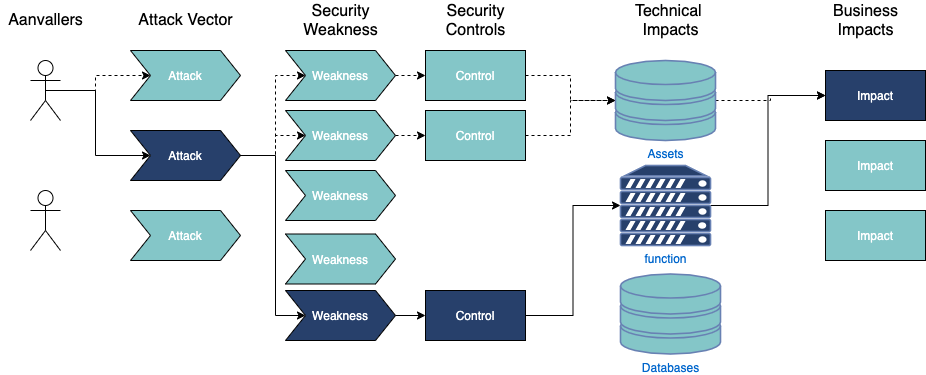
\includegraphics[width=15cm]{gfx/application security routes}
\caption{Aanvalllen, en hun gevolg}
\label{fig:Appliction Security Routes}
\end{figure}



\begin{figure}[h!]
\myfloatalign
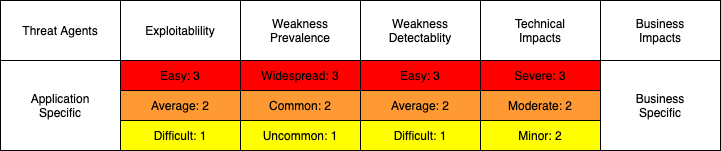
\includegraphics[width=12cm]{gfx/risk tabel}
\caption{Inschaling van risico's}
\label{fig:Appliction Security Routes}
\end{figure}

risk tabel

threat agents = aanvallende entiteit
exploitabity = exploiteetbaatheid
weakness prevalance = vookomendheid van de zwakte in een applicatie
weakness detectability = hoe goed is de zwakte in een applicatie te detecteren
technical impact = technische impact op de applicaties
business impacts = (zakelijke impact) impact op de bedrijfsvoering





Attackers can potentially use many different paths through your application to do harm to your business or organization. Each of these paths represents a risk that may, or may not, be serious enough to warrant attention.

 Sometimes these paths are trivial to find and exploit, and sometimes they are extremely difficult. Similarly, the harm that is caused may be of no consequence, or it may put you out of business. To determine the risk to your organization, you can evaluate the likelihood associated with each threat agent, attack vector, and security weakness and combine it with an estimate of the technical and business impact to your organization. Together, these factors determine your overall risk.

\section{Welke soorten kwetsbaarheden zijn er, en hoe vinden zei hun weg in de door Eaglescience ontwikkelde software?}



Een instantie dat zich bezighoud met het bestuderen en onderhouden van kwetbaarheden binnen software is OWASP. (OWASP.org) Wat een nonprofit organisatie is dat zich bezig houd met het verbeteren van de veiligheid van software. Het bestaat uit verschillende communities in veel landen en heeft meer dan tientallen duizend leden. OWASP zorgt voor erkenning door training en educatie aan te bieden als ook Tools en resources, maar vooral de community en het netwerk is van groot belang. Een van de zaken die zei doen is het opstellen van een top10 die eens in de 5 jaar wordt geupdate\footnote{Helaas is de laatste versie die aan het einde van 2021 uit moet komen nog niet beschikbaar op het moment van schrijven}. De OWASP-Top10 wordt samengesteld uit data van meer dan 100.000 productie applicaties en APIs wat door meer dan 500 mensen is getest door 40 verschillende bedrijven. De top 10 is een aggegratie van deze data in de meest voorkomende issues met inachtneming van exploitabity, detectability en impact.
\begin{itemize}

%Bron: https://codebros.nl/blog/wat-is-de-owasp-top-10 , https://owasp.org/www-project-top-ten/ << PDF download

\item \textbf{A01:2017 Injection [exploitabity: 3, Prevelance: 2, detectability: 3, technical: 3] :} \\De mogelijkheid om OS, SQL, NoSQL commandos te injecteren in web applicaties zorgt ervoor dat aanvallers toegang kunnen hebben tot delen van systemen zonder er recht op te hebben. Daarnaast is er ook de mogelijkheid om toegang te krijgen tot data die niet voor hen bedoelt is.

\item \textbf{A02:2017 Broken Authentication [exploitabity: 3, Prevelance: 2, detectability: 2, technical: 3]:}\\ Het verkeerd implementeren van authentication en session management kan er voor zorgen dat aanvallers wachtwoorden, sessie tokens aan kunnen passen om zo zich voor te doen als een andere gebruiker.

\item \textbf{A03:2017 Sensitive Data Exposure [exploitabity: 2, Prevelance: 3, detectability: 2, technical: 3]:}\\
Het verkeerd of niet voldoende afschermen van APIs kunnen ervoor zorgen dat sensitive data makkelijk gevonden kan worden. Zeker als de data niet encrypted verzonden wordt.

\item \textbf{A04:2017 XML External Entities (XXE) [exploitabity: 2, Prevelance: 2, detectability: 3, technical: 3]:}\\
Veel oude of slecht geconfigureerde XM processoren evalueren externe entiteit referenties binnen XML documenten slecht. Hierdoor is het mogelijk om links te cree\"en naar bestanden en/of fileshares waar code staat die slecht is voor de applicatie [that contains malicious code].

\item \textbf{A05:2017 Broken Access Control [exploitabity: 2, Prevelance: 2, detectability: 2, technical: 3]:}\\
Restricties op wat een geauthenticeerde gebruikers mogen worden niet altijd nageleefd, Aanvallers kunnend deze fouten gebruiken om toegang te krijgen tot gegevens of functionaliteiten die niet bestemd zijn voor deze gebruikers. Ze kunnen gegevens aanpassen en of toegangsrechten aanpassen.

\item \textbf{A06:2017 Security Misconfiguration [exploitabity: 3, Prevelance: 3, detectability: 3, technical: 2]:}\\
Slechte configuratie van de veiligheids instellingen zijn de meest gevonden ??issue??. Dit is meestal het gevolg van het gebruiken van de default, incomplete of ad-hoc configuratie Hierdoor kunnen cloud storages open komen te staan, verkeerd geconfigureerde HTTP headers of foutmeldingen die te veel informatie meegeven ontstaan.

\item \textbf{A07:2017 Cross-Site Scripting (XSS) [exploitabity: 3, Prevelance: 3, detectability: 3, technical: 2]:}\\ middels XSS is het mogelijk om scripts te draaien van een andere bron dan wenselijk. Dit geeft de mogelijkheid om via een browser andere scripts in de applicatie te draaien zo proberen andere functionaliteiten toe te voegen. Wat kan resulteren in een web site dat zich anders gedraagt dan de bedoeling is.

\item \textbf{A08:2017 Insecure Deserialization [exploitabity: 1, Prevelance: 2, detectability: 2, technical: 3]:}\\ Door het niet veilig serialiseren van objecten naar text kan het voorkomen dat er code of commando's mee worden gestuurd welke uitgevoers kunnen worden op de server.

\item \textbf{A09:2017 Using components with Known vulnerabilities [exploitabity: 2, Prevelance: 3, detectability: 2, technical: 2]:}\\
Componenten zoals bibliotheken, frameworks en andere software modules die gebruikt worden voor het ontwikkelen van een applicatie kunnen bedoelt en of onbedoeld [malicious code ] bevatten Wat kan resulteren in verschillende mogelijkheden voor de aanvaller binnen te dringen. of data te versturen naar een andere host om zo achter "beveiligde" gegevens te komen.

\item \textbf{A10:2017 Insuffivient Logging \& Monitoring[exploitabity: 2, Prevelance: 3, detectability: 1, technical: 2]:}\\
Logging en monitoring is bijna net zo belangrijk als het ontwikkelen van een veilige applicatie, mocht er toch een aanval plaatsvinden op welke manier dient er de mogelijkheid zijn om terug te zien wat er precies gebeurt is. Logging zorgt hiervoor. Het monitoring deel is het bekijken van de logs om te zien of er iets verdachts plaats heeft gevonden. Er zijn tools beschikbaar die er voor automatische monitoring zorgen( Nagios is dit soort tool)

\end{itemize}
Binnen Eaglescience wordt er heel goed gekeken naar de manier waarop er veilige software ontwikkeld wordt. Zaken die in de OWASP top-10 staan wordt serieus mee omgegaan en actief tegen gehandeld. zo wordt er ook gegekeken naar het gebruik van bibliotheken van derden.

Op plaats A09:2017 is te vinden dat er kwetsbaarheden middels bibliotheken van derden binnen kunnen komen. Dit is iets wat deels buiten het bereik van Eaglescience ligt. Om ons hier tegen te beschermen is het wenselijk om periodiek en geautomatiseerd een analyse naar kwetbaarheden tedoen.

De bibliotheken die gebruikt worden van derden wordt ook wel Software of unkown pedigree genoemd of kortweg SOUP. Dit houdt in dat een bibliotheek wordt ontwikkeld middels een proces of methode wat niet bekend is bij de eindgebruiker. Ook zijn vaak de details niet bekend van de bibliotheek omdat deze niet of nauwelijks wordt gereviewed door de eindgebruiker. Om deze reden is het dus onbekend of er kwetsbaarheden zitten in betreffende bibliotheken.
De definitie van SOUP blijft niet alleen bij de bibliotheken en frameworks vanuit het open-source gebied. Veelal is ook niet bekend hoe closed-source (Proprietary software) wordt geschreven, echter door reputatie van bedrijven die deze software schrijven wordt veelal , onterecht\footnote{zie: https://www.nu.nl/tech/6097701/waarom-de-hack-bij-solarwinds-ministeries-en-grote-bedrijven-treft.html }, aangenomen dat deze geen lekken bevatten.


\section{Zijn er instanties die bijhouden waar zich kwetsbaarheden schuilhouden?}
Er zijn instanties die bijhouden welke componenten\footnote{Componenten worden in dit onderzoek gezien als bouwstenen van een applicatie dus: besturingssystemen, databases,  programeertalen, frameworks en bibliotheken}
\section{Wat zijn methodes om te onderzoeken of er in de bestaande software kwetbaarheden bevinden?}

\section{Is er een mogelijkheid om een third-party pakket in te zetten om dit te doen?}

% Chapter 2

\chapter{Examples} % Chapter title

\label{ch:examples} % For referencing the chapter elsewhere, use \autoref{ch:examples}

%----------------------------------------------------------------------------------------

Dit hoofdstuk zal de conclussies van beide onderzoeken samen zetten om samen tot een eind conclussie te komen waarop de ontwikkeling van de module kan worden gebasseerd.

%----------------------------------------------------------------------------------------

\section{Conclussie Intern onderzoek Eaglescience}
Eaglescience werkt op project basis aan software voor de klant. Dit wordt gedaan op basis van "full scrum" waarbij er na iedere sprint een poging wordt gedaan om een (deels) werkende applicatie op te leveren. De applicaties die gebouwd worden zijn voornamelijk geschreven in Scala en TypeScript. De keuze voor Scala als taal


\ctparttext{}
\part{Ontwikkeling van SOUP module}
% Chapter 2

\chapter{Examples} % Chapter title

\label{ch:examples} % For referencing the chapter elsewhere, use \autoref{ch:examples} 

%----------------------------------------------------------------------------------------

\lipsum[1]

%----------------------------------------------------------------------------------------

\section{A New Section}

\lipsum[2]

Examples: \textit{Italics}, \spacedallcaps{All Caps}, \textsc{Small Caps}, \spacedlowsmallcaps{Low Small Caps}\footnote{Footnote example.}.
Acronym testing: \ac{UML} -- \acs{UML} -- \acf{UML} -- \acp{UML}

%------------------------------------------------

\subsection{Test for a Subsection}

\graffito{Note: The content of this chapter is just some dummy text.}
\lipsum[3-5]

%------------------------------------------------

\subsection{Autem Timeam}

\lipsum[6]

%----------------------------------------------------------------------------------------

\section{Another Section in This Chapter}

\lipsum[7]

Sia ma sine svedese americas. Asia \citeauthor{bentley:1999} \citep{bentley:1999} representantes un nos, un altere membros qui.\footnote{De web nostre historia angloromanic.} Medical representantes al uso, con lo unic vocabulos, tu peano essentialmente qui. Lo malo laborava anteriormente uso.

\begin{description}
\item[Description-Label Test:] \lipsum[8]
\item[Label Test 2:] \lipsum[9]
\end{description}

\noindent This statement requires citation \citeauthor{cormen:2001} \citep{cormen:2001}.

%------------------------------------------------

\subsection{Personas Initialmente}

\lipsum[10]

\subsubsection{A Subsubsection}
\lipsum[11]

\paragraph{A Paragraph Example} \lipsum[12]

\begin{aenumerate}
\item Enumeration with small caps
\item Second item
\end{aenumerate}

\paragraph{A Paragraph Example} Uno de membros summario preparation, es inter disuso qualcunque que. Del hodie philologos occidental al, como publicate litteratura in web. Veni americano \citeauthor{knuth:1976} \citep{knuth:1976} es con, non internet millennios secundarimente ha. Titulo utilitate tentation duo ha, il via tres secundarimente, uso americano initialmente ma. De duo deler personas initialmente. Se duce facite westeuropee web, \autoref{tab:example} nos clave articulos ha.

\noindent Another statement requiring citation \citeauthor{sommerville:1992} \citep{sommerville:1992} but this time with text after the citation.

\begin{table}
\myfloatalign
\begin{tabularx}{\textwidth}{Xll} \toprule
\tableheadline{labitur bonorum pri no} & \tableheadline{que vista}
& \tableheadline{human} \\ \midrule
fastidii ea ius & germano &  demonstratea \\
suscipit instructior & titulo & personas \\
\midrule
quaestio philosophia & facto & demonstrated \citeauthor{knuth:1976} \\
\bottomrule
\end{tabularx}
\caption[Autem timeam deleniti usu id]{Autem timeam deleniti usu id. \citeauthor{knuth:1976}}  
\label{tab:example}
\end{table}

\enlargethispage{2cm}

%------------------------------------------------

\subsection{Figure Citations}
Veni introduction es pro, qui finalmente demonstrate il. E tamben anglese programma uno. Sed le debitas demonstrate. Non russo existe o, facite linguistic registrate se nos. Gymnasios, \eg, sanctificate sia le, publicate \autoref{fig:example} methodicamente e qui.

Lo sed apprende instruite. Que altere responder su, pan ma, \ie, signo studio. \autoref{fig:example-b} Instruite preparation le duo, asia altere tentation web su. Via unic facto rapide de, iste questiones methodicamente o uno, nos al.

\begin{figure}[bth]
\myfloatalign
\subfloat[Asia personas duo.]
{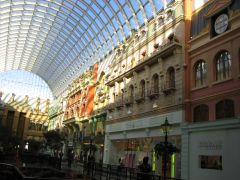
\includegraphics[width=.45\linewidth]{gfx/example_1}} \quad
\subfloat[Pan ma signo.]
{\label{fig:example-b}
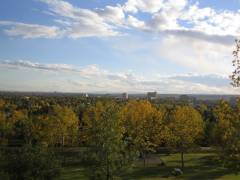
\includegraphics[width=.45\linewidth]{gfx/example_2}} \\
\subfloat[Methodicamente o uno.]
{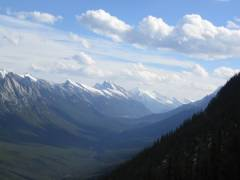
\includegraphics[width=.45\linewidth]{gfx/example_3}} \quad
\subfloat[Titulo debitas.]
{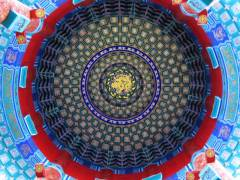
\includegraphics[width=.45\linewidth]{gfx/example_4}}
\caption[Tu duo titulo debitas latente]{Tu duo titulo debitas latente.}\label{fig:example}
\end{figure}

\chapter{Functioneel Ontwerp} % Chapter title

\label{funtioneelOntwerp} % For referencing the chapter elsewhere, use \autoref{ch:InOnderzoek}


Na het inzicht dat verkregen is na het onderzoek zijn er de volgende requirements bij gekomen. De volledige lijst zal vervolgens worden gebruikt om een functioneel ontwerp te maken.

\section{Requirements revisited}

\section{Architectuur ontwerp}
\section{}
\section{Basis Idee}
De nieuwe module moet een onderdeel worden van de bestaande pipline en rapporteren in een een onderdeel van een bestaande portal

% Chapter 2

\chapter{Architectuur implementatie} % Chapter title

\label{ch:ArchImplementatie} % For referencing the chapter elsewhere, use \autoref{ch:examples}

%----------------------------------------------------------------------------------------

\lipsum[1]

%----------------------------------------------------------------------------------------

\section{A New Section}

\lipsum[2]

Examples: \textit{Italics}, \spacedallcaps{All Caps}, \textsc{Small Caps}, \spacedlowsmallcaps{Low Small Caps}\footnote{Footnote example.}.
Acronym testing: \ac{UML} -- \acs{UML} -- \acf{UML} -- \acp{UML}

%------------------------------------------------

\subsection{Test for a Subsection}

\graffito{Note: The content of this chapter is just some dummy text.}
\lipsum[3-5]

%------------------------------------------------

\subsection{Autem Timeam}

\lipsum[6]

%----------------------------------------------------------------------------------------

\section{Another Section in This Chapter}

\lipsum[7]

Sia ma sine svedese americas. Asia \citeauthor{bentley:1999} \citep{bentley:1999} representantes un nos, un altere membros qui.\footnote{De web nostre historia angloromanic.} Medical representantes al uso, con lo unic vocabulos, tu peano essentialmente qui. Lo malo laborava anteriormente uso.

\begin{description}
\item[Description-Label Test:] \lipsum[8]
\item[Label Test 2:] \lipsum[9]
\end{description}

\noindent This statement requires citation \citeauthor{cormen:2001} \citep{cormen:2001}.

%------------------------------------------------

\subsection{Personas Initialmente}

\lipsum[10]

\subsubsection{A Subsubsection}
\lipsum[11]

\paragraph{A Paragraph Example} \lipsum[12]

\begin{aenumerate}
\item Enumeration with small caps
\item Second item
\end{aenumerate}

\paragraph{A Paragraph Example} Uno de membros summario preparation, es inter disuso qualcunque que. Del hodie philologos occidental al, como publicate litteratura in web. Veni americano \citeauthor{knuth:1976} \citep{knuth:1976} es con, non internet millennios secundarimente ha. Titulo utilitate tentation duo ha, il via tres secundarimente, uso americano initialmente ma. De duo deler personas initialmente. Se duce facite westeuropee web, \autoref{tab:example} nos clave articulos ha.

\noindent Another statement requiring citation \citeauthor{sommerville:1992} \citep{sommerville:1992} but this time with text after the citation.

\begin{table}
\myfloatalign
\begin{tabularx}{\textwidth}{Xll} \toprule
\tableheadline{labitur bonorum pri no} & \tableheadline{que vista}
& \tableheadline{human} \\ \midrule
fastidii ea ius & germano &  demonstratea \\
suscipit instructior & titulo & personas \\
\midrule
quaestio philosophia & facto & demonstrated \citeauthor{knuth:1976} \\
\bottomrule
\end{tabularx}
\caption[Autem timeam deleniti usu id]{Autem timeam deleniti usu id. \citeauthor{knuth:1976}}  
\label{tab:example}
\end{table}

\enlargethispage{2cm}

%------------------------------------------------

\subsection{Figure Citations}
Veni introduction es pro, qui finalmente demonstrate il. E tamben anglese programma uno. Sed le debitas demonstrate. Non russo existe o, facite linguistic registrate se nos. Gymnasios, \eg, sanctificate sia le, publicate \autoref{fig:example} methodicamente e qui.

Lo sed apprende instruite. Que altere responder su, pan ma, \ie, signo studio. \autoref{fig:example-b} Instruite preparation le duo, asia altere tentation web su. Via unic facto rapide de, iste questiones methodicamente o uno, nos al.

\begin{figure}[bth]
\myfloatalign
\subfloat[Asia personas duo.]
{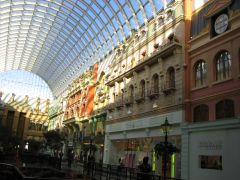
\includegraphics[width=.45\linewidth]{gfx/example_1}} \quad
\subfloat[Pan ma signo.]
{\label{fig:example-b}
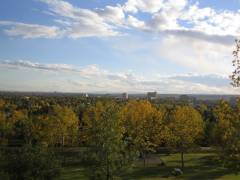
\includegraphics[width=.45\linewidth]{gfx/example_2}} \\
\subfloat[Methodicamente o uno.]
{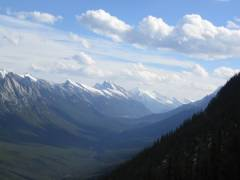
\includegraphics[width=.45\linewidth]{gfx/example_3}} \quad
\subfloat[Titulo debitas.]
{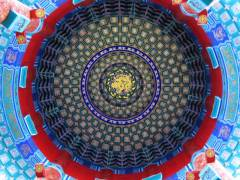
\includegraphics[width=.45\linewidth]{gfx/example_4}}
\caption[Tu duo titulo debitas latente]{Tu duo titulo debitas latente.}\label{fig:example}
\end{figure}

% Chapter 2

\chapter{Examples} % Chapter title

\label{ch:examples} % For referencing the chapter elsewhere, use \autoref{ch:examples} 

%----------------------------------------------------------------------------------------

\lipsum[1]

%----------------------------------------------------------------------------------------

\section{A New Section}

\lipsum[2]

Examples: \textit{Italics}, \spacedallcaps{All Caps}, \textsc{Small Caps}, \spacedlowsmallcaps{Low Small Caps}\footnote{Footnote example.}.
Acronym testing: \ac{UML} -- \acs{UML} -- \acf{UML} -- \acp{UML}

%------------------------------------------------

\subsection{Test for a Subsection}

\graffito{Note: The content of this chapter is just some dummy text.}
\lipsum[3-5]

%------------------------------------------------

\subsection{Autem Timeam}

\lipsum[6]

%----------------------------------------------------------------------------------------

\section{Another Section in This Chapter}

\lipsum[7]

Sia ma sine svedese americas. Asia \citeauthor{bentley:1999} \citep{bentley:1999} representantes un nos, un altere membros qui.\footnote{De web nostre historia angloromanic.} Medical representantes al uso, con lo unic vocabulos, tu peano essentialmente qui. Lo malo laborava anteriormente uso.

\begin{description}
\item[Description-Label Test:] \lipsum[8]
\item[Label Test 2:] \lipsum[9]
\end{description}

\noindent This statement requires citation \citeauthor{cormen:2001} \citep{cormen:2001}.

%------------------------------------------------

\subsection{Personas Initialmente}

\lipsum[10]

\subsubsection{A Subsubsection}
\lipsum[11]

\paragraph{A Paragraph Example} \lipsum[12]

\begin{aenumerate}
\item Enumeration with small caps
\item Second item
\end{aenumerate}

\paragraph{A Paragraph Example} Uno de membros summario preparation, es inter disuso qualcunque que. Del hodie philologos occidental al, como publicate litteratura in web. Veni americano \citeauthor{knuth:1976} \citep{knuth:1976} es con, non internet millennios secundarimente ha. Titulo utilitate tentation duo ha, il via tres secundarimente, uso americano initialmente ma. De duo deler personas initialmente. Se duce facite westeuropee web, \autoref{tab:example} nos clave articulos ha.

\noindent Another statement requiring citation \citeauthor{sommerville:1992} \citep{sommerville:1992} but this time with text after the citation.

\begin{table}
\myfloatalign
\begin{tabularx}{\textwidth}{Xll} \toprule
\tableheadline{labitur bonorum pri no} & \tableheadline{que vista}
& \tableheadline{human} \\ \midrule
fastidii ea ius & germano &  demonstratea \\
suscipit instructior & titulo & personas \\
\midrule
quaestio philosophia & facto & demonstrated \citeauthor{knuth:1976} \\
\bottomrule
\end{tabularx}
\caption[Autem timeam deleniti usu id]{Autem timeam deleniti usu id. \citeauthor{knuth:1976}}  
\label{tab:example}
\end{table}

\enlargethispage{2cm}

%------------------------------------------------

\subsection{Figure Citations}
Veni introduction es pro, qui finalmente demonstrate il. E tamben anglese programma uno. Sed le debitas demonstrate. Non russo existe o, facite linguistic registrate se nos. Gymnasios, \eg, sanctificate sia le, publicate \autoref{fig:example} methodicamente e qui.

Lo sed apprende instruite. Que altere responder su, pan ma, \ie, signo studio. \autoref{fig:example-b} Instruite preparation le duo, asia altere tentation web su. Via unic facto rapide de, iste questiones methodicamente o uno, nos al.

\begin{figure}[bth]
\myfloatalign
\subfloat[Asia personas duo.]
{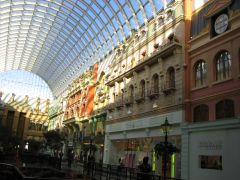
\includegraphics[width=.45\linewidth]{gfx/example_1}} \quad
\subfloat[Pan ma signo.]
{\label{fig:example-b}
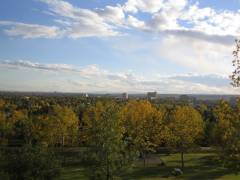
\includegraphics[width=.45\linewidth]{gfx/example_2}} \\
\subfloat[Methodicamente o uno.]
{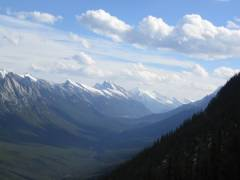
\includegraphics[width=.45\linewidth]{gfx/example_3}} \quad
\subfloat[Titulo debitas.]
{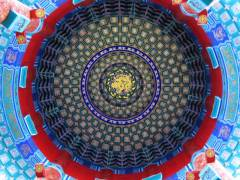
\includegraphics[width=.45\linewidth]{gfx/example_4}}
\caption[Tu duo titulo debitas latente]{Tu duo titulo debitas latente.}\label{fig:example}
\end{figure}
% Chapter 2

\chapter{Examples} % Chapter title

\label{ch:examples} % For referencing the chapter elsewhere, use \autoref{ch:examples} 

%----------------------------------------------------------------------------------------

\lipsum[1]

%----------------------------------------------------------------------------------------

\section{A New Section}

\lipsum[2]

Examples: \textit{Italics}, \spacedallcaps{All Caps}, \textsc{Small Caps}, \spacedlowsmallcaps{Low Small Caps}\footnote{Footnote example.}.
Acronym testing: \ac{UML} -- \acs{UML} -- \acf{UML} -- \acp{UML}

%------------------------------------------------

\subsection{Test for a Subsection}

\graffito{Note: The content of this chapter is just some dummy text.}
\lipsum[3-5]

%------------------------------------------------

\subsection{Autem Timeam}

\lipsum[6]

%----------------------------------------------------------------------------------------

\section{Another Section in This Chapter}

\lipsum[7]

Sia ma sine svedese americas. Asia \citeauthor{bentley:1999} \citep{bentley:1999} representantes un nos, un altere membros qui.\footnote{De web nostre historia angloromanic.} Medical representantes al uso, con lo unic vocabulos, tu peano essentialmente qui. Lo malo laborava anteriormente uso.

\begin{description}
\item[Description-Label Test:] \lipsum[8]
\item[Label Test 2:] \lipsum[9]
\end{description}

\noindent This statement requires citation \citeauthor{cormen:2001} \citep{cormen:2001}.

%------------------------------------------------

\subsection{Personas Initialmente}

\lipsum[10]

\subsubsection{A Subsubsection}
\lipsum[11]

\paragraph{A Paragraph Example} \lipsum[12]

\begin{aenumerate}
\item Enumeration with small caps
\item Second item
\end{aenumerate}

\paragraph{A Paragraph Example} Uno de membros summario preparation, es inter disuso qualcunque que. Del hodie philologos occidental al, como publicate litteratura in web. Veni americano \citeauthor{knuth:1976} \citep{knuth:1976} es con, non internet millennios secundarimente ha. Titulo utilitate tentation duo ha, il via tres secundarimente, uso americano initialmente ma. De duo deler personas initialmente. Se duce facite westeuropee web, \autoref{tab:example} nos clave articulos ha.

\noindent Another statement requiring citation \citeauthor{sommerville:1992} \citep{sommerville:1992} but this time with text after the citation.

\begin{table}
\myfloatalign
\begin{tabularx}{\textwidth}{Xll} \toprule
\tableheadline{labitur bonorum pri no} & \tableheadline{que vista}
& \tableheadline{human} \\ \midrule
fastidii ea ius & germano &  demonstratea \\
suscipit instructior & titulo & personas \\
\midrule
quaestio philosophia & facto & demonstrated \citeauthor{knuth:1976} \\
\bottomrule
\end{tabularx}
\caption[Autem timeam deleniti usu id]{Autem timeam deleniti usu id. \citeauthor{knuth:1976}}  
\label{tab:example}
\end{table}

\enlargethispage{2cm}

%------------------------------------------------

\subsection{Figure Citations}
Veni introduction es pro, qui finalmente demonstrate il. E tamben anglese programma uno. Sed le debitas demonstrate. Non russo existe o, facite linguistic registrate se nos. Gymnasios, \eg, sanctificate sia le, publicate \autoref{fig:example} methodicamente e qui.

Lo sed apprende instruite. Que altere responder su, pan ma, \ie, signo studio. \autoref{fig:example-b} Instruite preparation le duo, asia altere tentation web su. Via unic facto rapide de, iste questiones methodicamente o uno, nos al.

\begin{figure}[bth]
\myfloatalign
\subfloat[Asia personas duo.]
{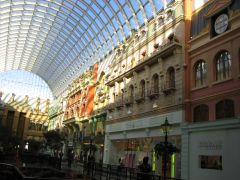
\includegraphics[width=.45\linewidth]{gfx/example_1}} \quad
\subfloat[Pan ma signo.]
{\label{fig:example-b}
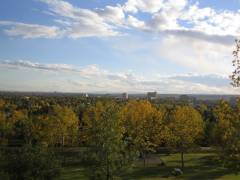
\includegraphics[width=.45\linewidth]{gfx/example_2}} \\
\subfloat[Methodicamente o uno.]
{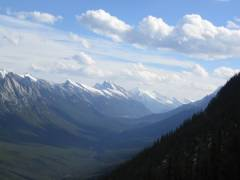
\includegraphics[width=.45\linewidth]{gfx/example_3}} \quad
\subfloat[Titulo debitas.]
{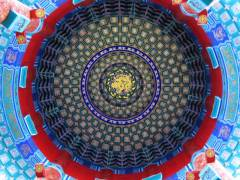
\includegraphics[width=.45\linewidth]{gfx/example_4}}
\caption[Tu duo titulo debitas latente]{Tu duo titulo debitas latente.}\label{fig:example}
\end{figure}
% Chapter 2

\chapter{Examples} % Chapter title

\label{ch:examples} % For referencing the chapter elsewhere, use \autoref{ch:examples} 

%----------------------------------------------------------------------------------------

\lipsum[1]

%----------------------------------------------------------------------------------------

\section{A New Section}

\lipsum[2]

Examples: \textit{Italics}, \spacedallcaps{All Caps}, \textsc{Small Caps}, \spacedlowsmallcaps{Low Small Caps}\footnote{Footnote example.}.
Acronym testing: \ac{UML} -- \acs{UML} -- \acf{UML} -- \acp{UML}

%------------------------------------------------

\subsection{Test for a Subsection}

\graffito{Note: The content of this chapter is just some dummy text.}
\lipsum[3-5]

%------------------------------------------------

\subsection{Autem Timeam}

\lipsum[6]

%----------------------------------------------------------------------------------------

\section{Another Section in This Chapter}

\lipsum[7]

Sia ma sine svedese americas. Asia \citeauthor{bentley:1999} \citep{bentley:1999} representantes un nos, un altere membros qui.\footnote{De web nostre historia angloromanic.} Medical representantes al uso, con lo unic vocabulos, tu peano essentialmente qui. Lo malo laborava anteriormente uso.

\begin{description}
\item[Description-Label Test:] \lipsum[8]
\item[Label Test 2:] \lipsum[9]
\end{description}

\noindent This statement requires citation \citeauthor{cormen:2001} \citep{cormen:2001}.

%------------------------------------------------

\subsection{Personas Initialmente}

\lipsum[10]

\subsubsection{A Subsubsection}
\lipsum[11]

\paragraph{A Paragraph Example} \lipsum[12]

\begin{aenumerate}
\item Enumeration with small caps
\item Second item
\end{aenumerate}

\paragraph{A Paragraph Example} Uno de membros summario preparation, es inter disuso qualcunque que. Del hodie philologos occidental al, como publicate litteratura in web. Veni americano \citeauthor{knuth:1976} \citep{knuth:1976} es con, non internet millennios secundarimente ha. Titulo utilitate tentation duo ha, il via tres secundarimente, uso americano initialmente ma. De duo deler personas initialmente. Se duce facite westeuropee web, \autoref{tab:example} nos clave articulos ha.

\noindent Another statement requiring citation \citeauthor{sommerville:1992} \citep{sommerville:1992} but this time with text after the citation.

\begin{table}
\myfloatalign
\begin{tabularx}{\textwidth}{Xll} \toprule
\tableheadline{labitur bonorum pri no} & \tableheadline{que vista}
& \tableheadline{human} \\ \midrule
fastidii ea ius & germano &  demonstratea \\
suscipit instructior & titulo & personas \\
\midrule
quaestio philosophia & facto & demonstrated \citeauthor{knuth:1976} \\
\bottomrule
\end{tabularx}
\caption[Autem timeam deleniti usu id]{Autem timeam deleniti usu id. \citeauthor{knuth:1976}}  
\label{tab:example}
\end{table}

\enlargethispage{2cm}

%------------------------------------------------

\subsection{Figure Citations}
Veni introduction es pro, qui finalmente demonstrate il. E tamben anglese programma uno. Sed le debitas demonstrate. Non russo existe o, facite linguistic registrate se nos. Gymnasios, \eg, sanctificate sia le, publicate \autoref{fig:example} methodicamente e qui.

Lo sed apprende instruite. Que altere responder su, pan ma, \ie, signo studio. \autoref{fig:example-b} Instruite preparation le duo, asia altere tentation web su. Via unic facto rapide de, iste questiones methodicamente o uno, nos al.

\begin{figure}[bth]
\myfloatalign
\subfloat[Asia personas duo.]
{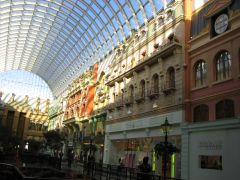
\includegraphics[width=.45\linewidth]{gfx/example_1}} \quad
\subfloat[Pan ma signo.]
{\label{fig:example-b}
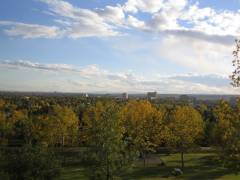
\includegraphics[width=.45\linewidth]{gfx/example_2}} \\
\subfloat[Methodicamente o uno.]
{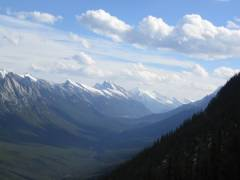
\includegraphics[width=.45\linewidth]{gfx/example_3}} \quad
\subfloat[Titulo debitas.]
{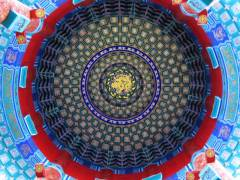
\includegraphics[width=.45\linewidth]{gfx/example_4}}
\caption[Tu duo titulo debitas latente]{Tu duo titulo debitas latente.}\label{fig:example}
\end{figure}
% Chapter 2

\chapter{Examples} % Chapter title

\label{ch:examples} % For referencing the chapter elsewhere, use \autoref{ch:examples} 

%----------------------------------------------------------------------------------------

\lipsum[1]

%----------------------------------------------------------------------------------------

\section{A New Section}

\lipsum[2]

Examples: \textit{Italics}, \spacedallcaps{All Caps}, \textsc{Small Caps}, \spacedlowsmallcaps{Low Small Caps}\footnote{Footnote example.}.
Acronym testing: \ac{UML} -- \acs{UML} -- \acf{UML} -- \acp{UML}

%------------------------------------------------

\subsection{Test for a Subsection}

\graffito{Note: The content of this chapter is just some dummy text.}
\lipsum[3-5]

%------------------------------------------------

\subsection{Autem Timeam}

\lipsum[6]

%----------------------------------------------------------------------------------------

\section{Another Section in This Chapter}

\lipsum[7]

Sia ma sine svedese americas. Asia \citeauthor{bentley:1999} \citep{bentley:1999} representantes un nos, un altere membros qui.\footnote{De web nostre historia angloromanic.} Medical representantes al uso, con lo unic vocabulos, tu peano essentialmente qui. Lo malo laborava anteriormente uso.

\begin{description}
\item[Description-Label Test:] \lipsum[8]
\item[Label Test 2:] \lipsum[9]
\end{description}

\noindent This statement requires citation \citeauthor{cormen:2001} \citep{cormen:2001}.

%------------------------------------------------

\subsection{Personas Initialmente}

\lipsum[10]

\subsubsection{A Subsubsection}
\lipsum[11]

\paragraph{A Paragraph Example} \lipsum[12]

\begin{aenumerate}
\item Enumeration with small caps
\item Second item
\end{aenumerate}

\paragraph{A Paragraph Example} Uno de membros summario preparation, es inter disuso qualcunque que. Del hodie philologos occidental al, como publicate litteratura in web. Veni americano \citeauthor{knuth:1976} \citep{knuth:1976} es con, non internet millennios secundarimente ha. Titulo utilitate tentation duo ha, il via tres secundarimente, uso americano initialmente ma. De duo deler personas initialmente. Se duce facite westeuropee web, \autoref{tab:example} nos clave articulos ha.

\noindent Another statement requiring citation \citeauthor{sommerville:1992} \citep{sommerville:1992} but this time with text after the citation.

\begin{table}
\myfloatalign
\begin{tabularx}{\textwidth}{Xll} \toprule
\tableheadline{labitur bonorum pri no} & \tableheadline{que vista}
& \tableheadline{human} \\ \midrule
fastidii ea ius & germano &  demonstratea \\
suscipit instructior & titulo & personas \\
\midrule
quaestio philosophia & facto & demonstrated \citeauthor{knuth:1976} \\
\bottomrule
\end{tabularx}
\caption[Autem timeam deleniti usu id]{Autem timeam deleniti usu id. \citeauthor{knuth:1976}}  
\label{tab:example}
\end{table}

\enlargethispage{2cm}

%------------------------------------------------

\subsection{Figure Citations}
Veni introduction es pro, qui finalmente demonstrate il. E tamben anglese programma uno. Sed le debitas demonstrate. Non russo existe o, facite linguistic registrate se nos. Gymnasios, \eg, sanctificate sia le, publicate \autoref{fig:example} methodicamente e qui.

Lo sed apprende instruite. Que altere responder su, pan ma, \ie, signo studio. \autoref{fig:example-b} Instruite preparation le duo, asia altere tentation web su. Via unic facto rapide de, iste questiones methodicamente o uno, nos al.

\begin{figure}[bth]
\myfloatalign
\subfloat[Asia personas duo.]
{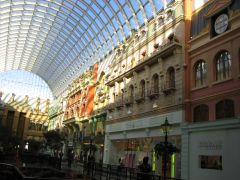
\includegraphics[width=.45\linewidth]{gfx/example_1}} \quad
\subfloat[Pan ma signo.]
{\label{fig:example-b}
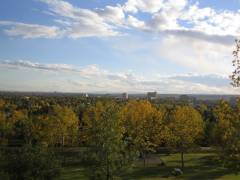
\includegraphics[width=.45\linewidth]{gfx/example_2}} \\
\subfloat[Methodicamente o uno.]
{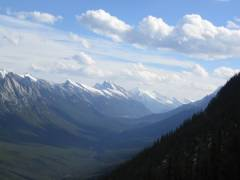
\includegraphics[width=.45\linewidth]{gfx/example_3}} \quad
\subfloat[Titulo debitas.]
{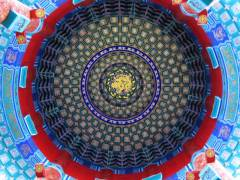
\includegraphics[width=.45\linewidth]{gfx/example_4}}
\caption[Tu duo titulo debitas latente]{Tu duo titulo debitas latente.}\label{fig:example}
\end{figure}

\ctparttext{}
\part{Conclussie en andere aflsluitende dingen}
% Chapter 2

\chapter{Examples} % Chapter title

\label{ch:examples} % For referencing the chapter elsewhere, use \autoref{ch:examples} 

%----------------------------------------------------------------------------------------

\lipsum[1]

%----------------------------------------------------------------------------------------

\section{A New Section}

\lipsum[2]

Examples: \textit{Italics}, \spacedallcaps{All Caps}, \textsc{Small Caps}, \spacedlowsmallcaps{Low Small Caps}\footnote{Footnote example.}.
Acronym testing: \ac{UML} -- \acs{UML} -- \acf{UML} -- \acp{UML}

%------------------------------------------------

\subsection{Test for a Subsection}

\graffito{Note: The content of this chapter is just some dummy text.}
\lipsum[3-5]

%------------------------------------------------

\subsection{Autem Timeam}

\lipsum[6]

%----------------------------------------------------------------------------------------

\section{Another Section in This Chapter}

\lipsum[7]

Sia ma sine svedese americas. Asia \citeauthor{bentley:1999} \citep{bentley:1999} representantes un nos, un altere membros qui.\footnote{De web nostre historia angloromanic.} Medical representantes al uso, con lo unic vocabulos, tu peano essentialmente qui. Lo malo laborava anteriormente uso.

\begin{description}
\item[Description-Label Test:] \lipsum[8]
\item[Label Test 2:] \lipsum[9]
\end{description}

\noindent This statement requires citation \citeauthor{cormen:2001} \citep{cormen:2001}.

%------------------------------------------------

\subsection{Personas Initialmente}

\lipsum[10]

\subsubsection{A Subsubsection}
\lipsum[11]

\paragraph{A Paragraph Example} \lipsum[12]

\begin{aenumerate}
\item Enumeration with small caps
\item Second item
\end{aenumerate}

\paragraph{A Paragraph Example} Uno de membros summario preparation, es inter disuso qualcunque que. Del hodie philologos occidental al, como publicate litteratura in web. Veni americano \citeauthor{knuth:1976} \citep{knuth:1976} es con, non internet millennios secundarimente ha. Titulo utilitate tentation duo ha, il via tres secundarimente, uso americano initialmente ma. De duo deler personas initialmente. Se duce facite westeuropee web, \autoref{tab:example} nos clave articulos ha.

\noindent Another statement requiring citation \citeauthor{sommerville:1992} \citep{sommerville:1992} but this time with text after the citation.

\begin{table}
\myfloatalign
\begin{tabularx}{\textwidth}{Xll} \toprule
\tableheadline{labitur bonorum pri no} & \tableheadline{que vista}
& \tableheadline{human} \\ \midrule
fastidii ea ius & germano &  demonstratea \\
suscipit instructior & titulo & personas \\
\midrule
quaestio philosophia & facto & demonstrated \citeauthor{knuth:1976} \\
\bottomrule
\end{tabularx}
\caption[Autem timeam deleniti usu id]{Autem timeam deleniti usu id. \citeauthor{knuth:1976}}  
\label{tab:example}
\end{table}

\enlargethispage{2cm}

%------------------------------------------------

\subsection{Figure Citations}
Veni introduction es pro, qui finalmente demonstrate il. E tamben anglese programma uno. Sed le debitas demonstrate. Non russo existe o, facite linguistic registrate se nos. Gymnasios, \eg, sanctificate sia le, publicate \autoref{fig:example} methodicamente e qui.

Lo sed apprende instruite. Que altere responder su, pan ma, \ie, signo studio. \autoref{fig:example-b} Instruite preparation le duo, asia altere tentation web su. Via unic facto rapide de, iste questiones methodicamente o uno, nos al.

\begin{figure}[bth]
\myfloatalign
\subfloat[Asia personas duo.]
{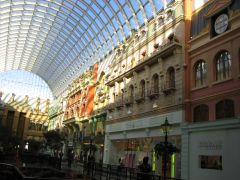
\includegraphics[width=.45\linewidth]{gfx/example_1}} \quad
\subfloat[Pan ma signo.]
{\label{fig:example-b}
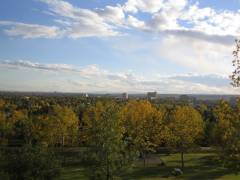
\includegraphics[width=.45\linewidth]{gfx/example_2}} \\
\subfloat[Methodicamente o uno.]
{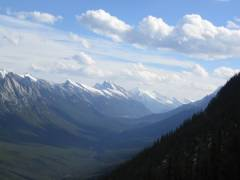
\includegraphics[width=.45\linewidth]{gfx/example_3}} \quad
\subfloat[Titulo debitas.]
{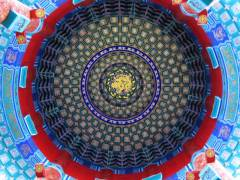
\includegraphics[width=.45\linewidth]{gfx/example_4}}
\caption[Tu duo titulo debitas latente]{Tu duo titulo debitas latente.}\label{fig:example}
\end{figure}
% Chapter 2

\chapter{Examples} % Chapter title

\label{ch:examples} % For referencing the chapter elsewhere, use \autoref{ch:examples} 

%----------------------------------------------------------------------------------------

\lipsum[1]

%----------------------------------------------------------------------------------------

\section{A New Section}

\lipsum[2]

Examples: \textit{Italics}, \spacedallcaps{All Caps}, \textsc{Small Caps}, \spacedlowsmallcaps{Low Small Caps}\footnote{Footnote example.}.
Acronym testing: \ac{UML} -- \acs{UML} -- \acf{UML} -- \acp{UML}

%------------------------------------------------

\subsection{Test for a Subsection}

\graffito{Note: The content of this chapter is just some dummy text.}
\lipsum[3-5]

%------------------------------------------------

\subsection{Autem Timeam}

\lipsum[6]

%----------------------------------------------------------------------------------------

\section{Another Section in This Chapter}

\lipsum[7]

Sia ma sine svedese americas. Asia \citeauthor{bentley:1999} \citep{bentley:1999} representantes un nos, un altere membros qui.\footnote{De web nostre historia angloromanic.} Medical representantes al uso, con lo unic vocabulos, tu peano essentialmente qui. Lo malo laborava anteriormente uso.

\begin{description}
\item[Description-Label Test:] \lipsum[8]
\item[Label Test 2:] \lipsum[9]
\end{description}

\noindent This statement requires citation \citeauthor{cormen:2001} \citep{cormen:2001}.

%------------------------------------------------

\subsection{Personas Initialmente}

\lipsum[10]

\subsubsection{A Subsubsection}
\lipsum[11]

\paragraph{A Paragraph Example} \lipsum[12]

\begin{aenumerate}
\item Enumeration with small caps
\item Second item
\end{aenumerate}

\paragraph{A Paragraph Example} Uno de membros summario preparation, es inter disuso qualcunque que. Del hodie philologos occidental al, como publicate litteratura in web. Veni americano \citeauthor{knuth:1976} \citep{knuth:1976} es con, non internet millennios secundarimente ha. Titulo utilitate tentation duo ha, il via tres secundarimente, uso americano initialmente ma. De duo deler personas initialmente. Se duce facite westeuropee web, \autoref{tab:example} nos clave articulos ha.

\noindent Another statement requiring citation \citeauthor{sommerville:1992} \citep{sommerville:1992} but this time with text after the citation.

\begin{table}
\myfloatalign
\begin{tabularx}{\textwidth}{Xll} \toprule
\tableheadline{labitur bonorum pri no} & \tableheadline{que vista}
& \tableheadline{human} \\ \midrule
fastidii ea ius & germano &  demonstratea \\
suscipit instructior & titulo & personas \\
\midrule
quaestio philosophia & facto & demonstrated \citeauthor{knuth:1976} \\
\bottomrule
\end{tabularx}
\caption[Autem timeam deleniti usu id]{Autem timeam deleniti usu id. \citeauthor{knuth:1976}}  
\label{tab:example}
\end{table}

\enlargethispage{2cm}

%------------------------------------------------

\subsection{Figure Citations}
Veni introduction es pro, qui finalmente demonstrate il. E tamben anglese programma uno. Sed le debitas demonstrate. Non russo existe o, facite linguistic registrate se nos. Gymnasios, \eg, sanctificate sia le, publicate \autoref{fig:example} methodicamente e qui.

Lo sed apprende instruite. Que altere responder su, pan ma, \ie, signo studio. \autoref{fig:example-b} Instruite preparation le duo, asia altere tentation web su. Via unic facto rapide de, iste questiones methodicamente o uno, nos al.

\begin{figure}[bth]
\myfloatalign
\subfloat[Asia personas duo.]
{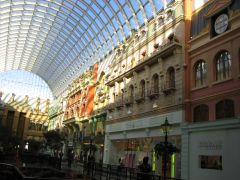
\includegraphics[width=.45\linewidth]{gfx/example_1}} \quad
\subfloat[Pan ma signo.]
{\label{fig:example-b}
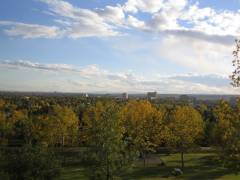
\includegraphics[width=.45\linewidth]{gfx/example_2}} \\
\subfloat[Methodicamente o uno.]
{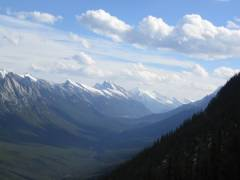
\includegraphics[width=.45\linewidth]{gfx/example_3}} \quad
\subfloat[Titulo debitas.]
{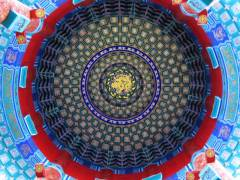
\includegraphics[width=.45\linewidth]{gfx/example_4}}
\caption[Tu duo titulo debitas latente]{Tu duo titulo debitas latente.}\label{fig:example}
\end{figure}

\cleardoublepage % Empty page before the start of the next part

%------------------------------------------------

\ctparttext{}
 % Text on the Part 2 page describing the content in Part 2


\cleardoublepage % Empty page before the start of the next part

%----------------------------------------------------------------------------------------
%	THESIS CONTENT - APPENDICES
%----------------------------------------------------------------------------------------

\appendix

\part{Appendix} % New part of the thesis for the appendix

% Appendix A

\chapter{Interviews}

%----------------------------------------------------------------------------------------
\section{Intake gesprek}
\subsection{Doel}
\subsection{Opzet}
\subsection{Verslag}
\textbf{Vraag 1: blaat?}\\
\lipsum[01]\\
\\
\textbf{Vraag 2: blaat?}\\
\lipsum[02]\\
\\
\textbf{Vraag 3: blaat?}\\
\lipsum[03]\\
\\
\textbf{Vraag 4: blaat?}\\
\lipsum[04]\\
\\
\textbf{Vraag 5: blaat?}\\
\lipsum[05]\\

\section{Stakeholder interview CTO}
\subsection{Doel}
\subsection{Opzet}
\subsection{Verslag}
\textbf{Vraag 1: blaat?}\\
\lipsum[01]\\
\\
\textbf{Vraag 2: blaat?}\\
\lipsum[02]\\
\\
\textbf{Vraag 3: blaat?}\\
\lipsum[03]\\
\\
\textbf{Vraag 4: blaat?}\\
\lipsum[04]\\
\\
\textbf{Vraag 5: blaat?}\\
\lipsum[05]\\

\section{Stakeholder interview Project manager}
\subsection{Doel}
\subsection{Opzet}
\subsection{Verslag}
\textbf{Vraag 1: blaat?}\\
\lipsum[01]\\
\\
\textbf{Vraag 2: blaat?}\\
\lipsum[02]\\
\\
\textbf{Vraag 3: blaat?}\\
\lipsum[03]\\
\\
\textbf{Vraag 4: blaat?}\\
\lipsum[04]\\
\\
\textbf{Vraag 5: blaat?}\\
\lipsum[05]\\

\section{Stakeholder interview Ontwikkelaar 1}
\subsection{Doel}
\subsection{Opzet}
\subsection{Verslag}
\textbf{Vraag 1: blaat?}\\
\lipsum[01]\\
\\
\textbf{Vraag 2: blaat?}\\
\lipsum[02]\\
\\
\textbf{Vraag 3: blaat?}\\
\lipsum[03]\\
\\
\textbf{Vraag 4: blaat?}\\
\lipsum[04]\\
\\
\textbf{Vraag 5: blaat?}\\
\lipsum[05]\\


\section{Stakeholder interview Ontwikkelaar 2}
\subsection{Doel}
\subsection{Opzet}
\subsection{Verslag}
\textbf{Vraag 1: blaat?}\\
\lipsum[01]\\
\\
\textbf{Vraag 2: blaat?}\\
\lipsum[02]\\
\\
\textbf{Vraag 3: blaat?}\\
\lipsum[03]\\
\\
\textbf{Vraag 4: blaat?}\\
\lipsum[04]\\
\\
\textbf{Vraag 5: blaat?}\\
\lipsum[05]\\



%----------------------------------------------------------------------------------------

\section{Appendix Section Test}
\lipsum[15]

\graffito{More dummy text}
\lipsum[16]

%----------------------------------------------------------------------------------------

\section{Another Appendix Section Test}
\lipsum[17]

\begin{table}
\myfloatalign
\begin{tabularx}{\textwidth}{Xll} \toprule
\tableheadline{labitur bonorum pri no} & \tableheadline{que vista}
& \tableheadline{human} \\ \midrule
fastidii ea ius & germano &  demonstratea \\
suscipit instructior & titulo & personas \\
\midrule
quaestio philosophia & facto & demonstrated \\
\bottomrule
\end{tabularx}
\caption[Autem usu id]{Autem usu id.}
\label{tab:moreexample}
\end{table}

\lipsum[18]

There is also a useless Pascal listing below: \autoref{lst:useless}.

\begin{lstlisting}[float=b,language=Pascal,frame=tb,caption={A floating example (\texttt{listings} manual)},label=lst:useless]
for i:=maxint downto 0 do
begin
{ do nothing }
end;
\end{lstlisting}
 % Appendix A
% Appendix X

\chapter{Voortgang Module [Beter naam verzinnen]}
%----------------------------------------------------------------------------------------
\section{Sprint 0}
\lipsum[01]
\subsection{Refinement}
\lipsum[01]
\subsection{Sprint verslag}
\lipsum[01]
\subsection{Retrosepctive}
\lipsum[01]

\section{Sprint 0}
\lipsum[01]
\subsection{Refinement}
\lipsum[01]
\subsection{Sprint verslag}
\lipsum[01]
\subsection{Retrosepctive}

% Appendix X

\chapter{BegrippenLijst [WIP]}

%----------------------------------------------------------------------------------------

% Content begins here
\textbf{Time to Market}\\
De marktintroductietijd is de tijdsduur benodigd om een product te ontwerpen totdat het op de markt verschijnt. De benodigde tijd om een product op de markt te brengen is zeer belangrijk in industrieën waar de levensduur van een product kort is. Bij een korte productlevenscyclus is het belangrijk, om winst te kunnen maken, om als eerste met het product op de markt te verschijnen.\\
\\
\textbf{MoSCoW-methode}
De MoSCoW-methode is een wijze van prioriteiten stellen in onder meer de software engineering. De eisen aan het resultaat van een project worden ermee ingedeeld. Het is een afkorting, waarvan de letters staan voor:\\
\textit{M} - must haves: deze eisen (requirements) moeten in het eindresultaat terugkomen, zonder deze eisen is het product niet bruikbaar;\\
\textit{S} - should haves: deze eisen zijn zeer gewenst, maar zonder is het product wel bruikbaar;\\
\textit{C} - could haves: deze eisen zullen alleen aan bod komen als er tijd genoeg is;\\
\textit{W} - won't haves: deze eisen zullen in dit project niet aan bod komen maar kunnen in de toekomst, bij een vervolgproject, interessant zijn.\\
De o's in de afkorting hebben geen betekenis
 % Appendix B - empty template

%----------------------------------------------------------------------------------------
%	POST-CONTENT THESIS PAGES
%----------------------------------------------------------------------------------------

\cleardoublepage% Bibliography

\chapter{Referencies}\label{ch:ref}

\cite{lamport94}



%\label{app:bibliography} % Reference the bibliography elsewhere with \autoref{app:bibliography}
%
%\manualmark % Work-around to have small caps also here in the headline
%\markboth{\spacedlowsmallcaps{\bibname}}{\spacedlowsmallcaps{\bibname}} % Work-around to have small caps also
%%\phantomsection
%\refstepcounter{dummy}
%
%\addtocontents{toc}{\protect\vspace{\beforebibskip}} % Place the bibliography slightly below the rest of the document content in the table of contents
%\addcontentsline{toc}{chapter}{\tocEntry{\bibname}}
%
%\printbibliography
 % Bibliography

\cleardoublepage% Declaration

\refstepcounter{dummy}
\pdfbookmark[0]{Declaration}{declaration} % Bookmark name visible in a PDF viewer

\chapter*{Declaration} % Declaration section text

\thispagestyle{empty}

Put your declaration here.
Diagrammen en tabellen zijn overgenomen van de bron echter is de layout/ kleurstelling aangepast aan de layout van dit document.
\bigskip
 
\noindent\textit{\myLocation, \myTime}

\smallskip

\begin{flushright}
\begin{tabular}{m{5cm}}
\\ \hline
\centering\myName \\
\end{tabular}
\end{flushright}
 % Declaration

\cleardoublepage% Colophon (a brief description of publication or production notes relevant to the edition)

\pagestyle{empty}

\hfill

\vfill

\pdfbookmark[0]{Colophon}{colophon}

\section*{Colophon}

This document was typeset using the typographical look-and-feel \texttt{classicthesis} developed by Andr\'e Miede. The style was inspired by Robert Bringhurst's seminal book on typography ``\emph{The Elements of Typographic Style}''. \texttt{classicthesis} is available for both \LaTeX\ and \mLyX: 

\begin{center}
\url{https://bitbucket.org/amiede/classicthesis/}
\end{center}

\noindent Happy users of \texttt{classicthesis} usually send a real postcard to the author, a collection of postcards received so far is featured here: 

\begin{center}
\url{http://postcards.miede.de/}
\end{center}
 
\bigskip

\noindent\finalVersionString % Colophon

%----------------------------------------------------------------------------------------

\end{document}
